\subsection{MVP}
$\indent$Để quan sát rõ hơn, thầy (cô) có thể truy cập:
\begin{itemize}
    \item \textbf{Link Figma:} \href{https://www.figma.com/file/5qWJujcpWwfKIJF0e06Z6T/SSPS?type=design&node-id=301%3A72&mode=design&t=VMGUT2u3DHGPAgda-1}{Xem tại đây}
    \item \textbf{Link Prototype:} \href{https://www.figma.com/proto/5qWJujcpWwfKIJF0e06Z6T/SSPS?node-id=424-16842&starting-point-node-id=361%3A12861&scaling=scale-down&mode=design&t=E1CTNMqU0qKDA57Y-1}{Xem tại đây}
\end{itemize}
\subsubsection{Trang chủ}
\begin{figure}[H]
    \begin{center}
        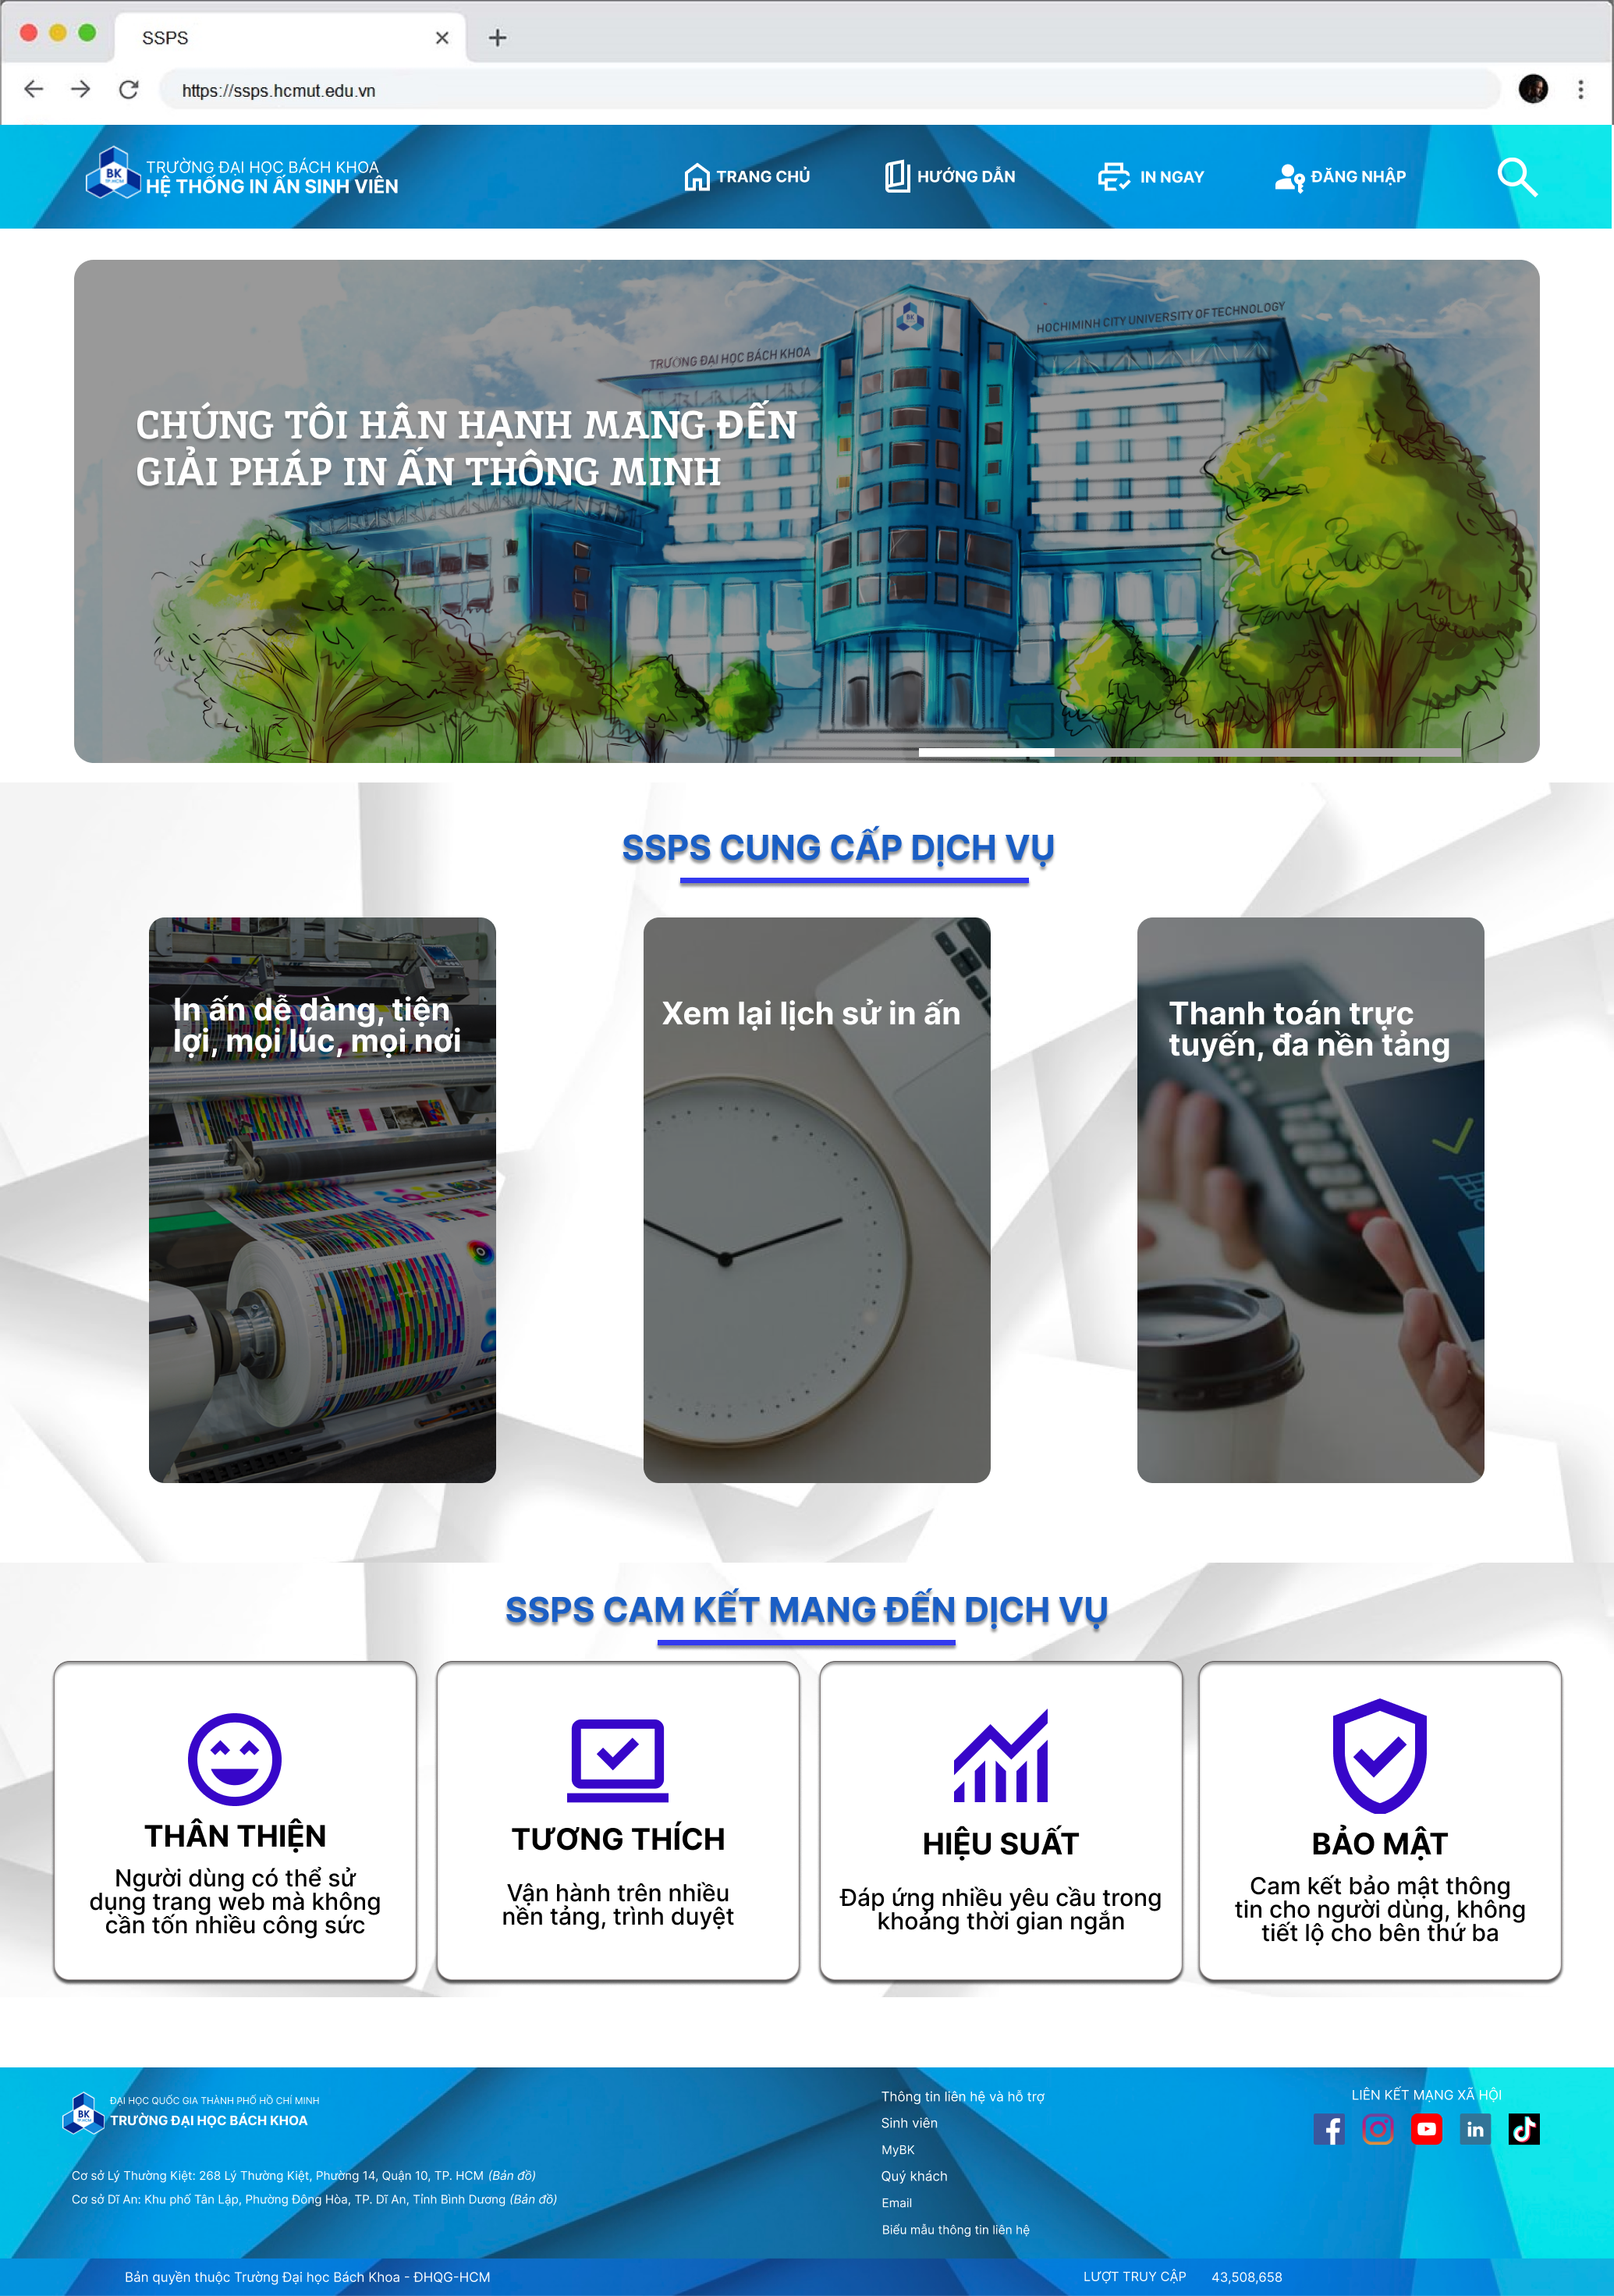
\includegraphics[width=0.8\textwidth]{Images/Figma/Homepage.png}
        \caption{Giao diện trang chủ cho khách}
        \label{fig:arch}
    \end{center}
\end{figure}
\begin{figure}[H]
    \begin{center}
        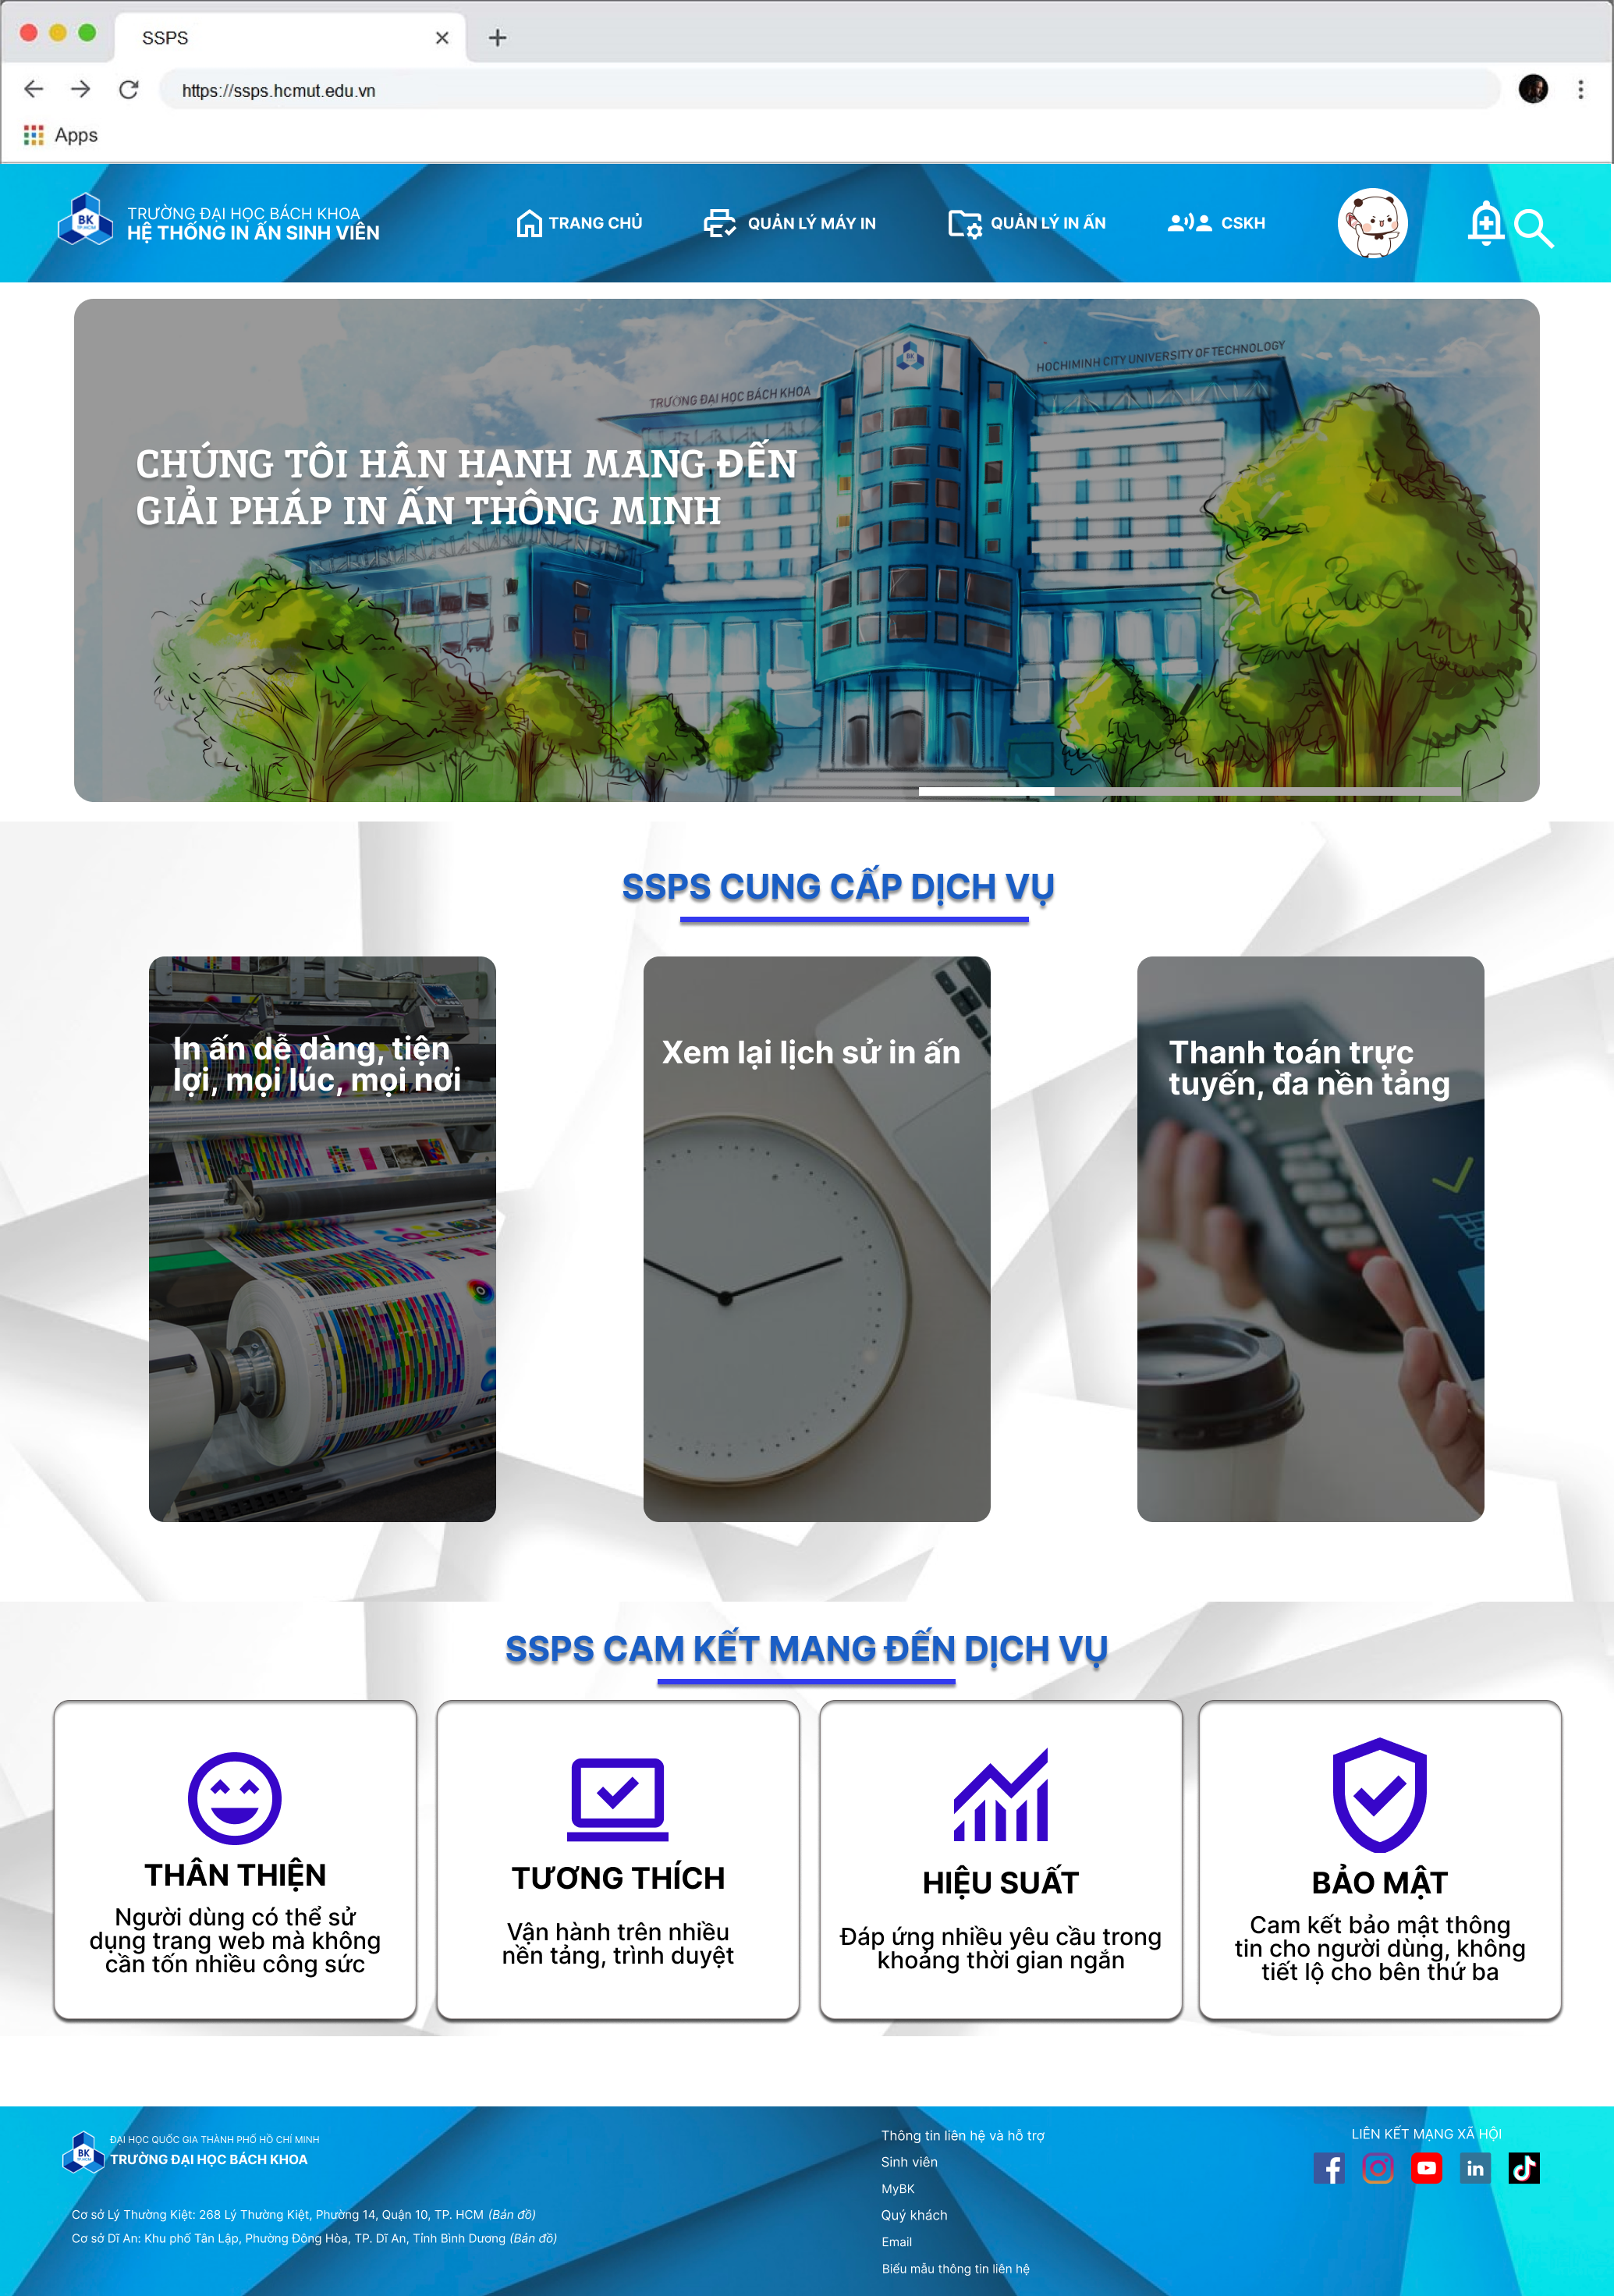
\includegraphics[width=0.8\textwidth]{Images/Figma/Homepage_spso.png}
        \caption{Giao diện trang chủ cho SPSO gồm Quản lý in ấn, máy in và CSKH}
        \label{fig:arch}
    \end{center}
\end{figure}
\begin{figure}[H]
    \begin{center}
        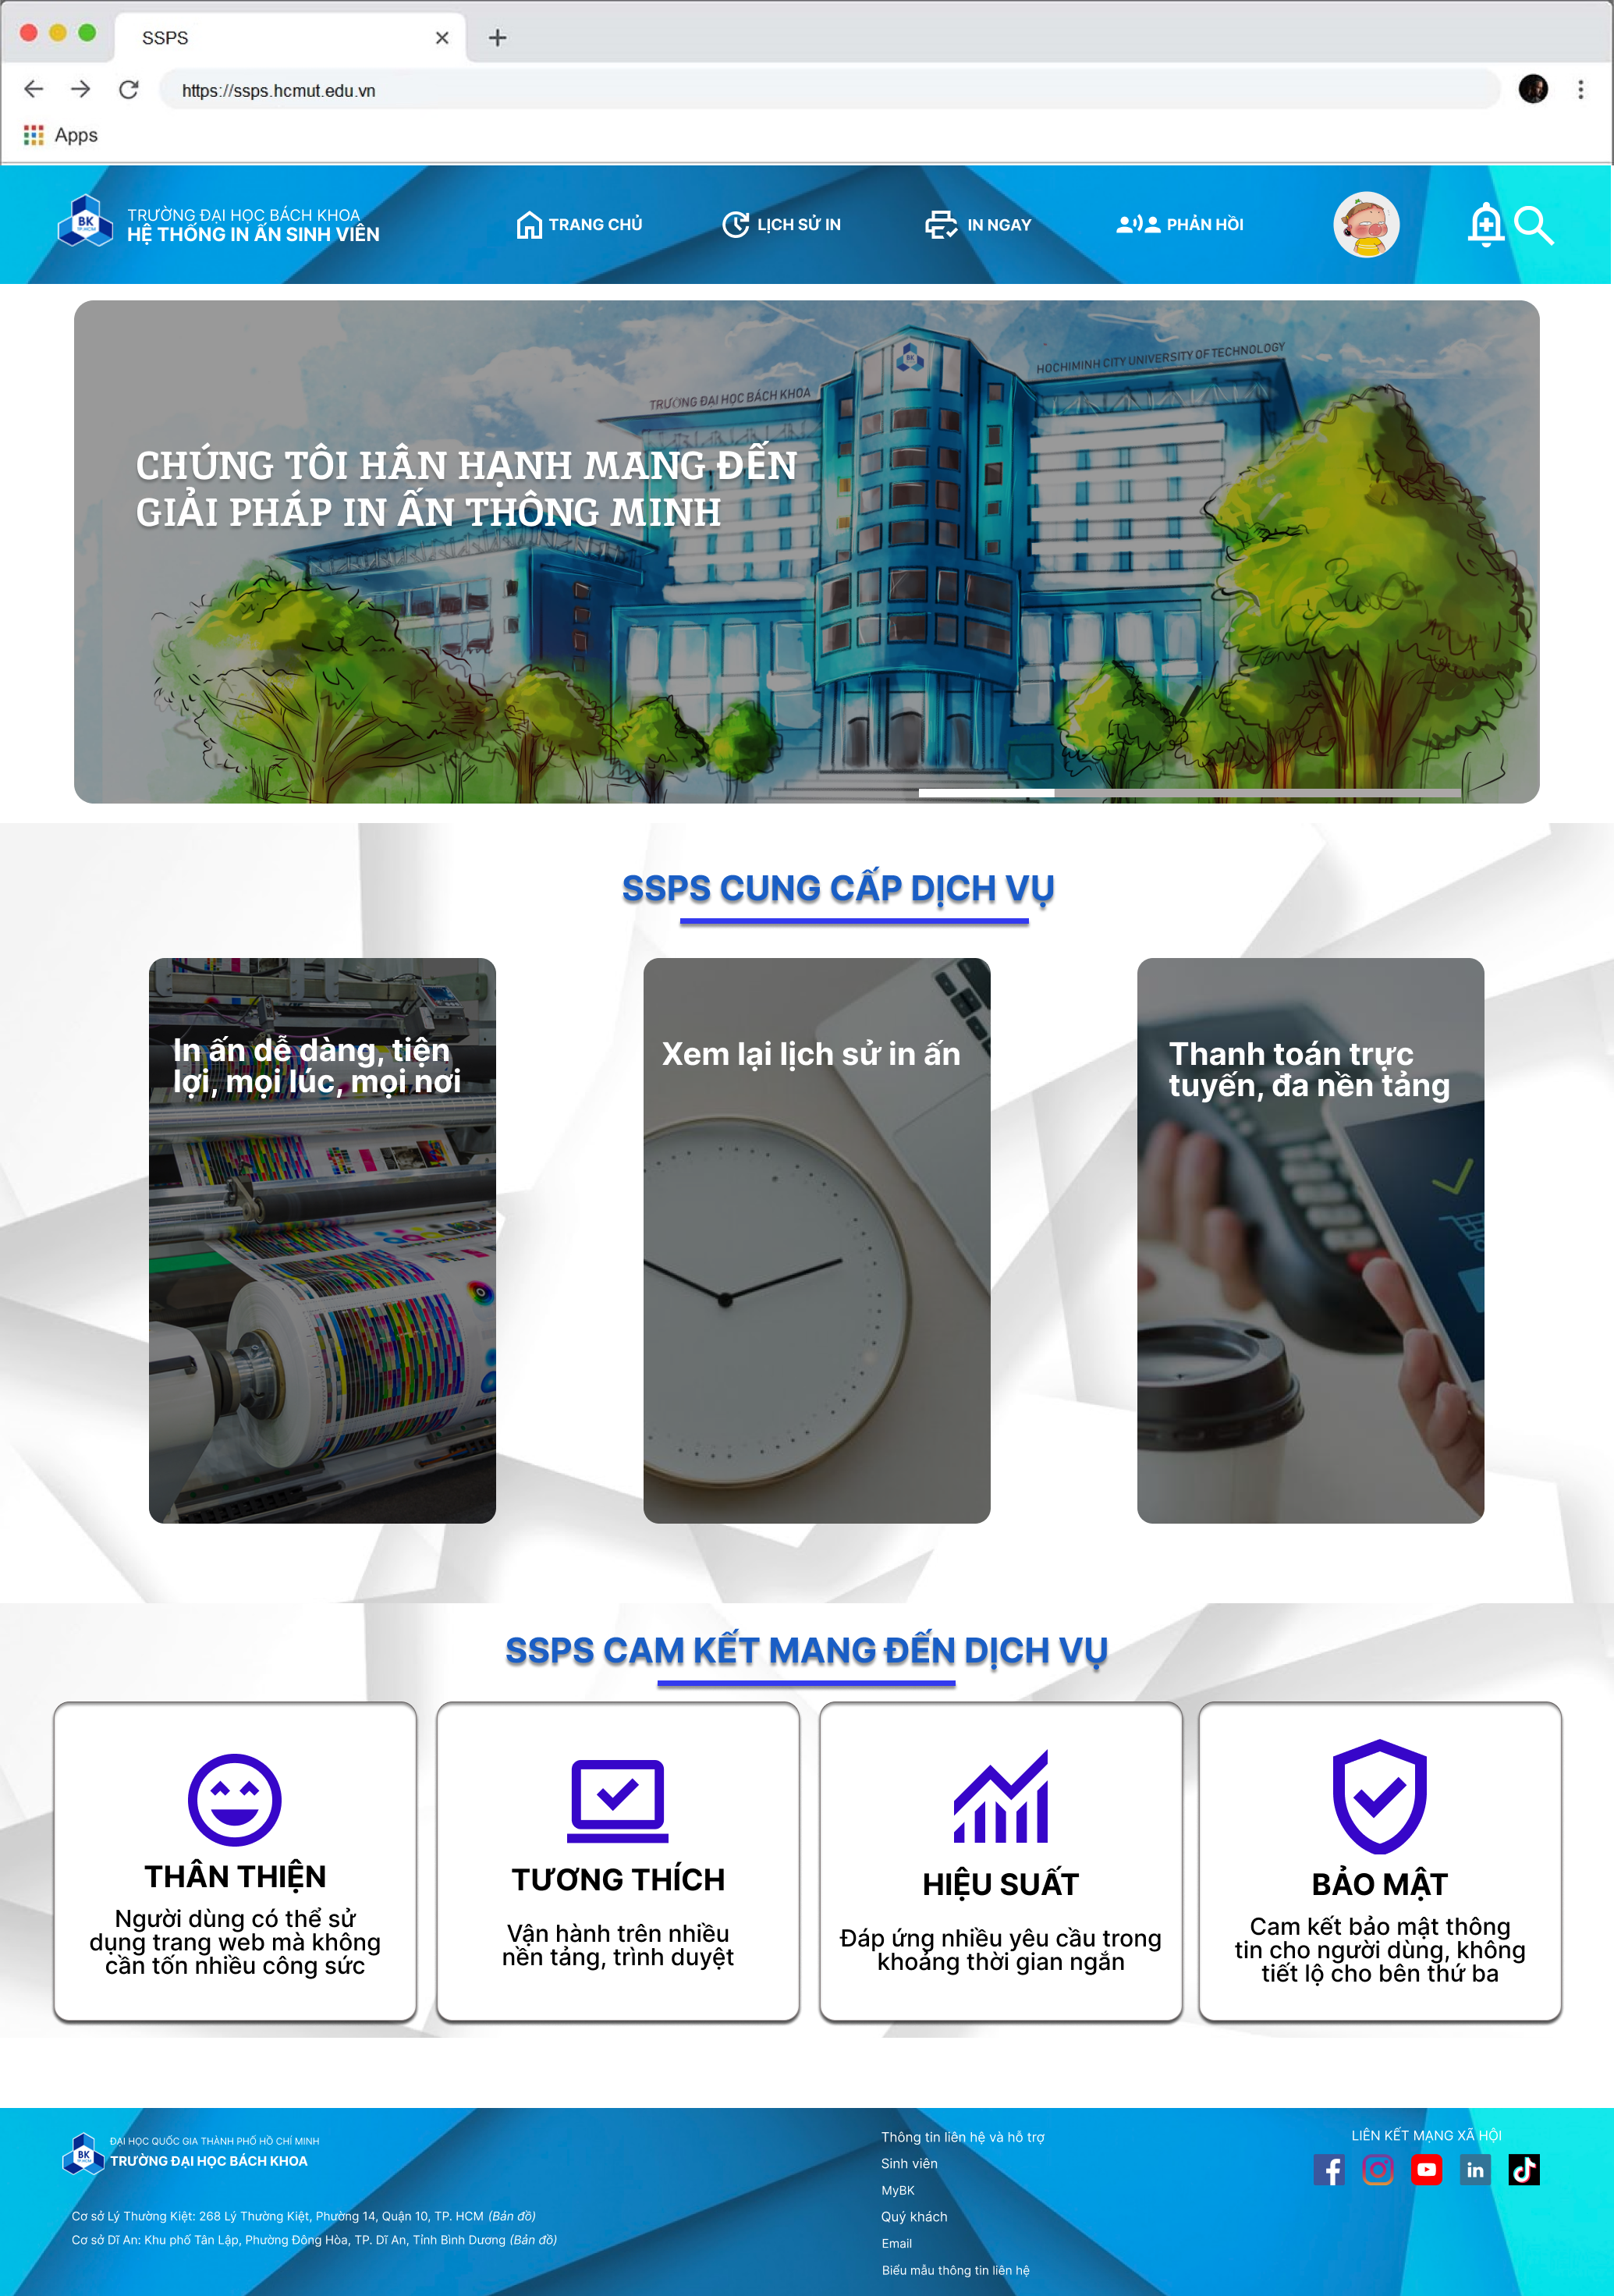
\includegraphics[width=0.8\textwidth]{Images/Figma/Homepage_stu.png}
        \caption{Giao diện trang chủ cho khách hàng gồm In ngay, Lịch sử in và Phản hồi}
        \label{fig:arch}
    \end{center}
\end{figure}
\subsubsection{Đăng nhập}
\begin{figure}[H]
    \begin{center}
        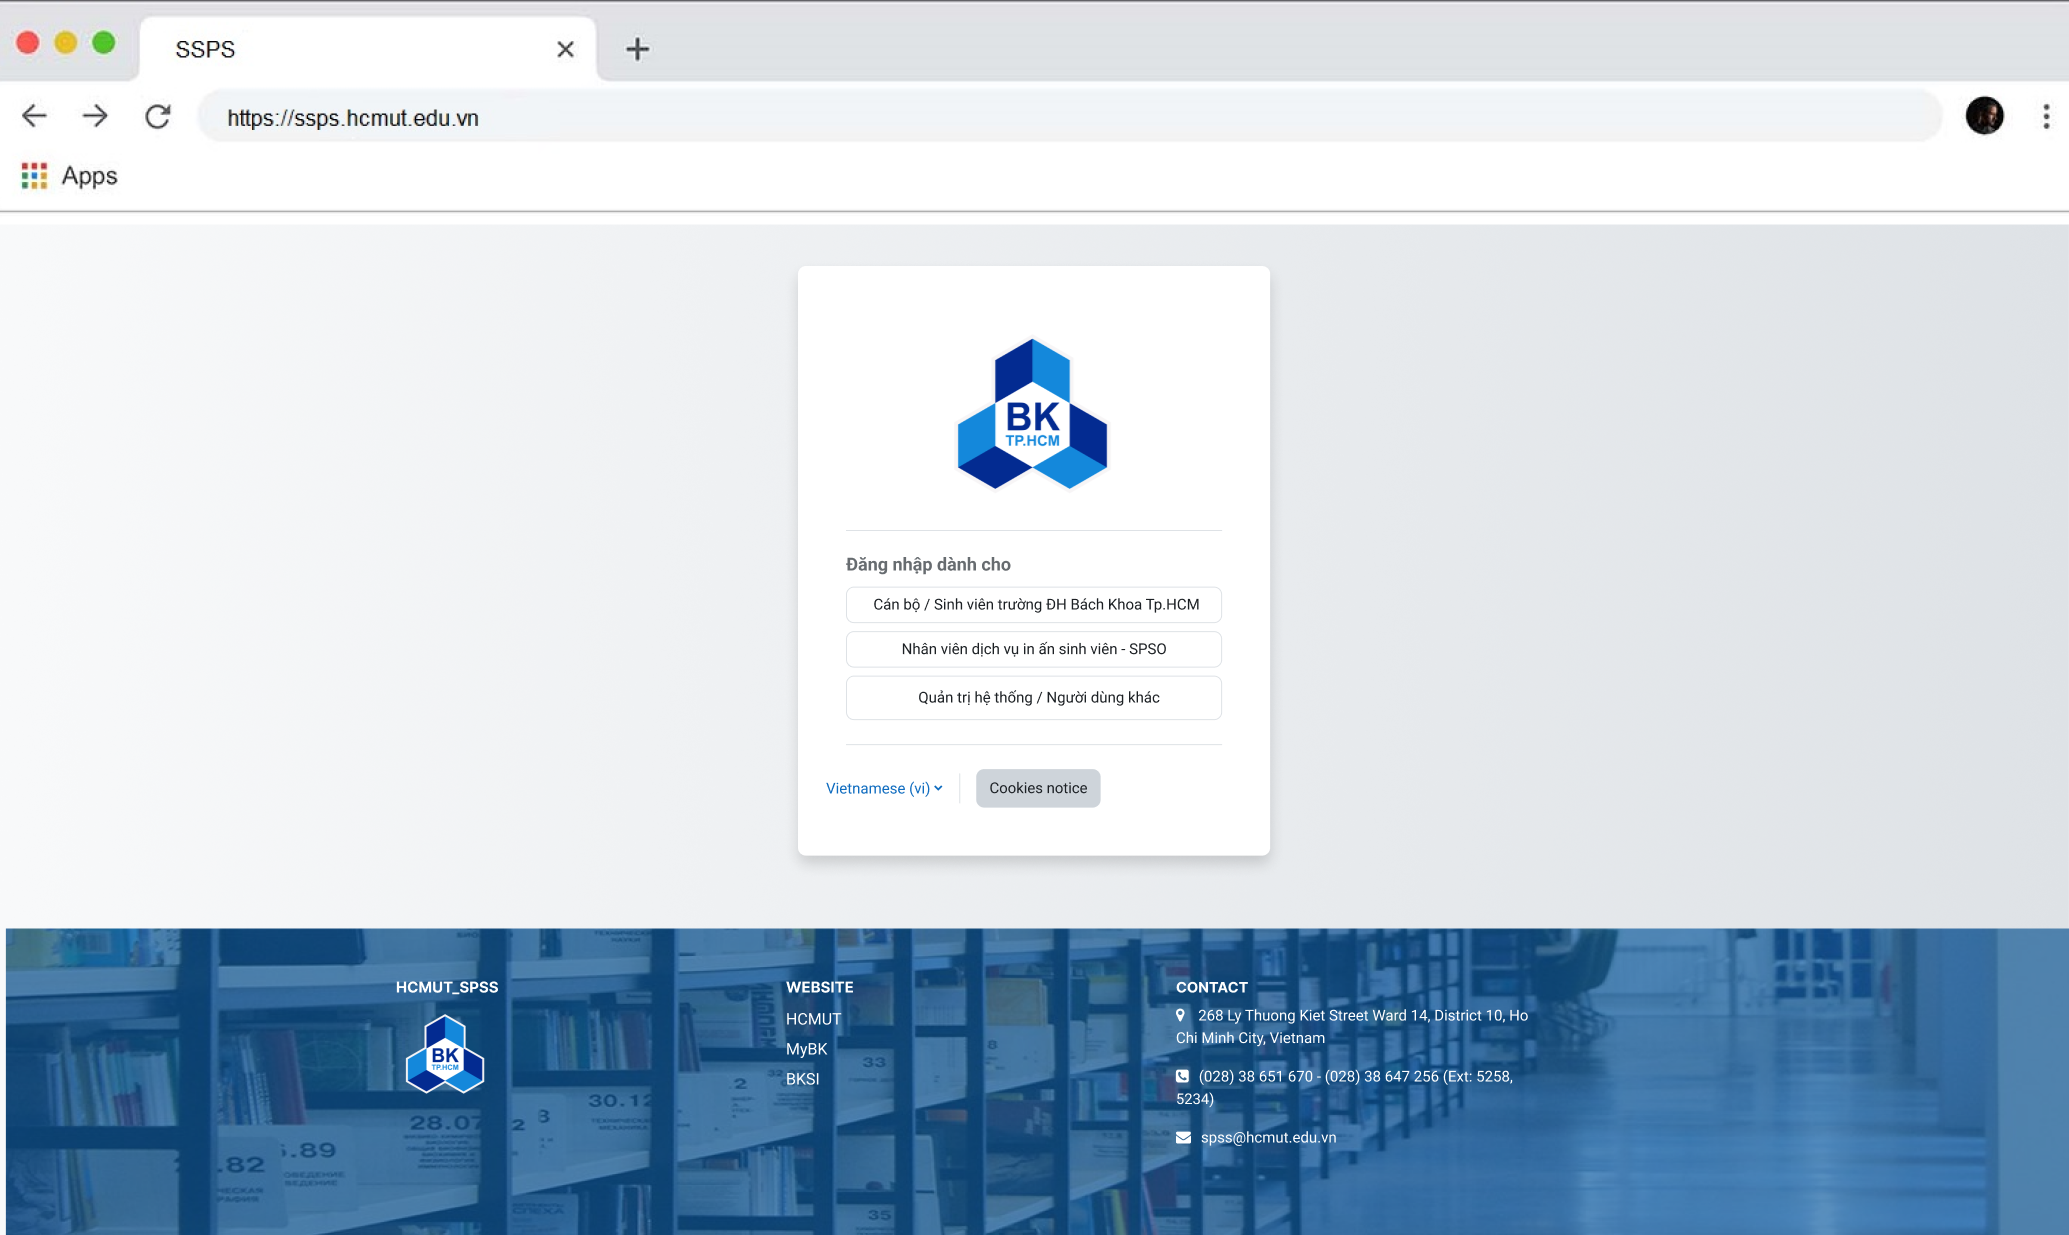
\includegraphics[width=1\textwidth]{Images/Figma/Login-Role.png}
        \caption{Giao diện đăng nhập (tham khảo từ BKeL)}
        \label{fig:arch}
    \end{center}
\end{figure}
$\indent$- Chọn vai trò là sinh viên hoặc cán bộ hoặc SPSO sau đó trang web sẽ chuyển hướng tới dịch vụ xác thực tập trung CAS HCMUT\_SSO của trường.
\subsubsection{In}
\begin{figure}[H]
    \begin{center}
        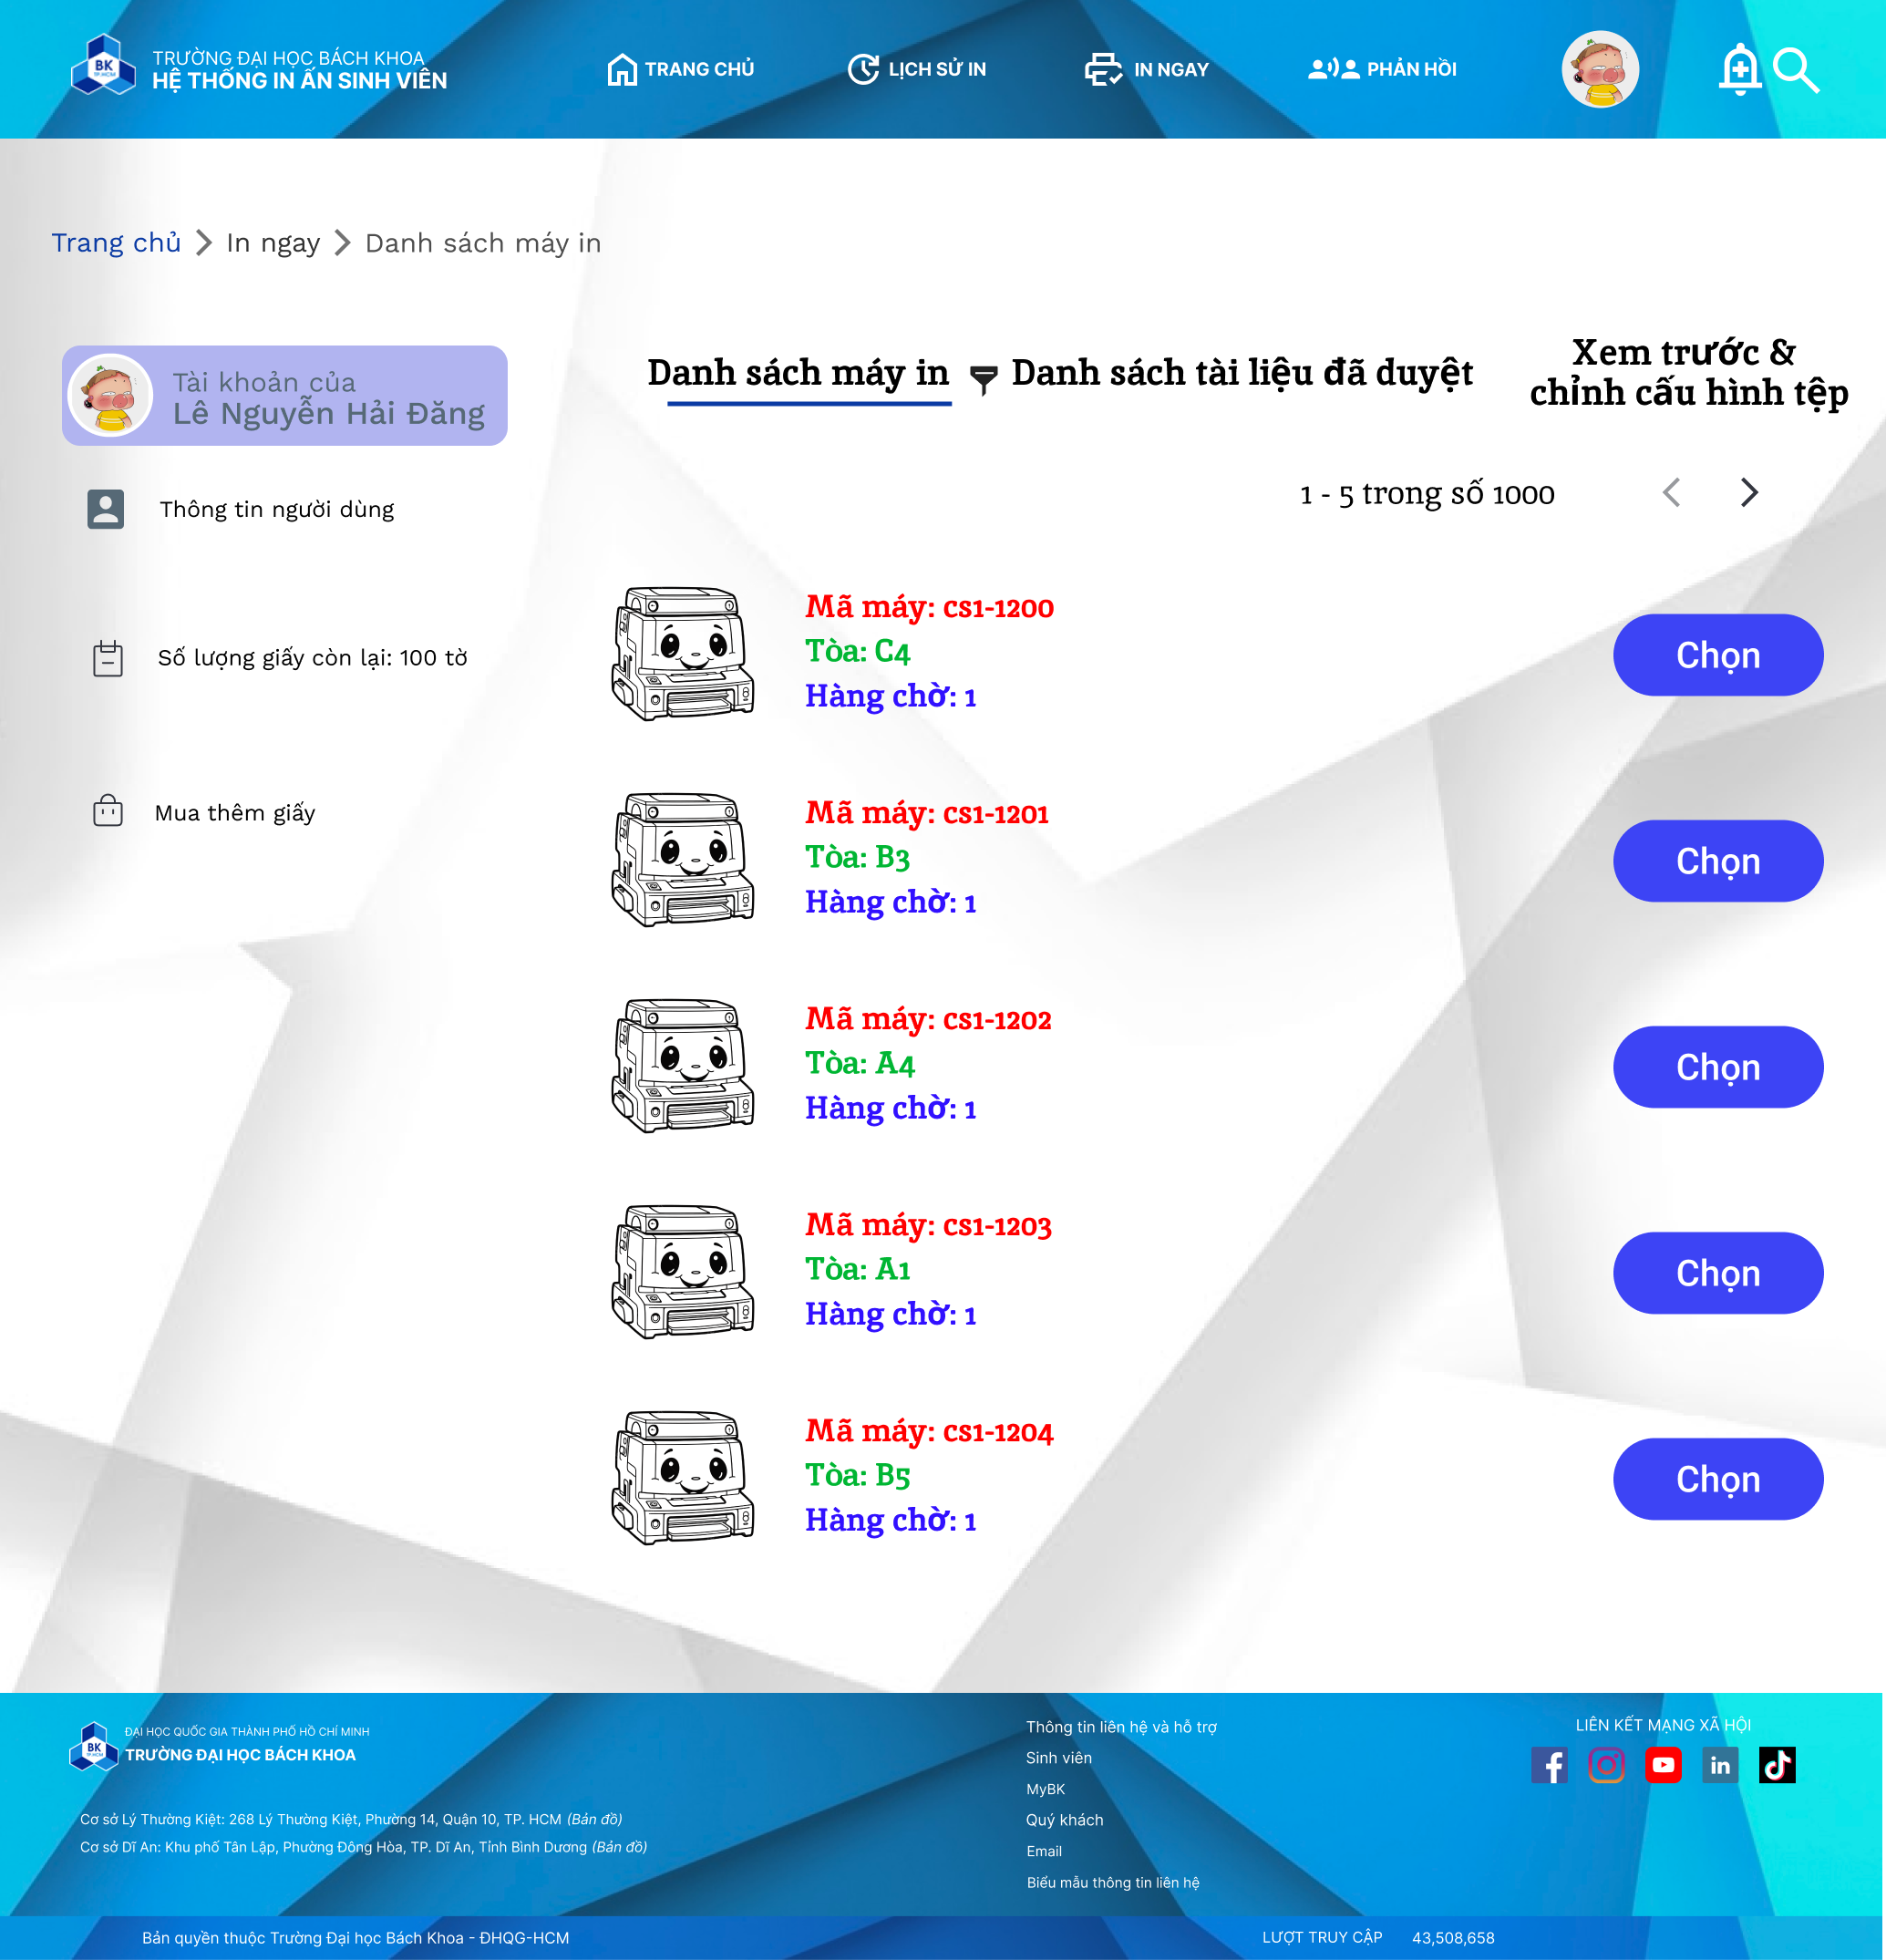
\includegraphics[width=1\textwidth]{Images/Figma/In ngay.png}
        \caption{Giao diện in cho khách hàng}
        \label{fig:arch}
    \end{center}
\end{figure}
$\indent$- Tại giao diện chọn máy in, khách hàng có thể chọn máy in theo danh sách hoặc dùng bộ lọc. Sau đó sẽ upload tài liệu lên website để chờ duyệt được in.
\begin{figure}[H]
    \begin{center}
        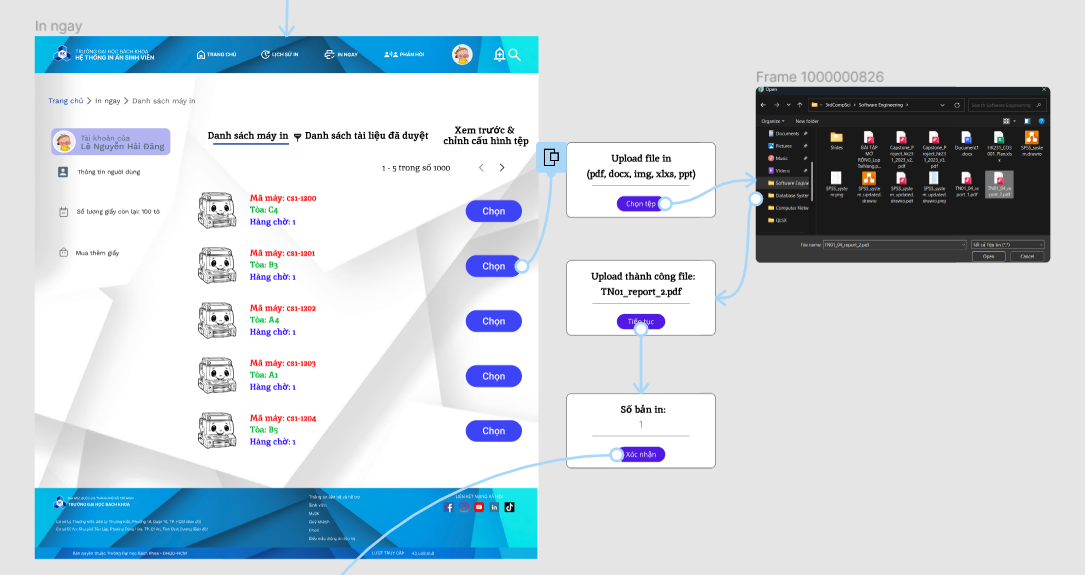
\includegraphics[width=1\textwidth]{Images/Figma/Inngay-upload.png}
        \caption{Mock-up chọn và upload }
        \label{fig:arch}
    \end{center}
\end{figure}
$\indent$- Nếu tài liệu upload đã được kiểm duyệt sẽ hiện thông báo và hiển thị tại \textbf{Danh sách đã duyệt} \\
$\indent$- Xem và cấu hình file trước khi in bằng cách ấn vào sidebar "Xem và chỉnh cấu hình tệp".
\begin{figure}[H]
    \begin{center}
        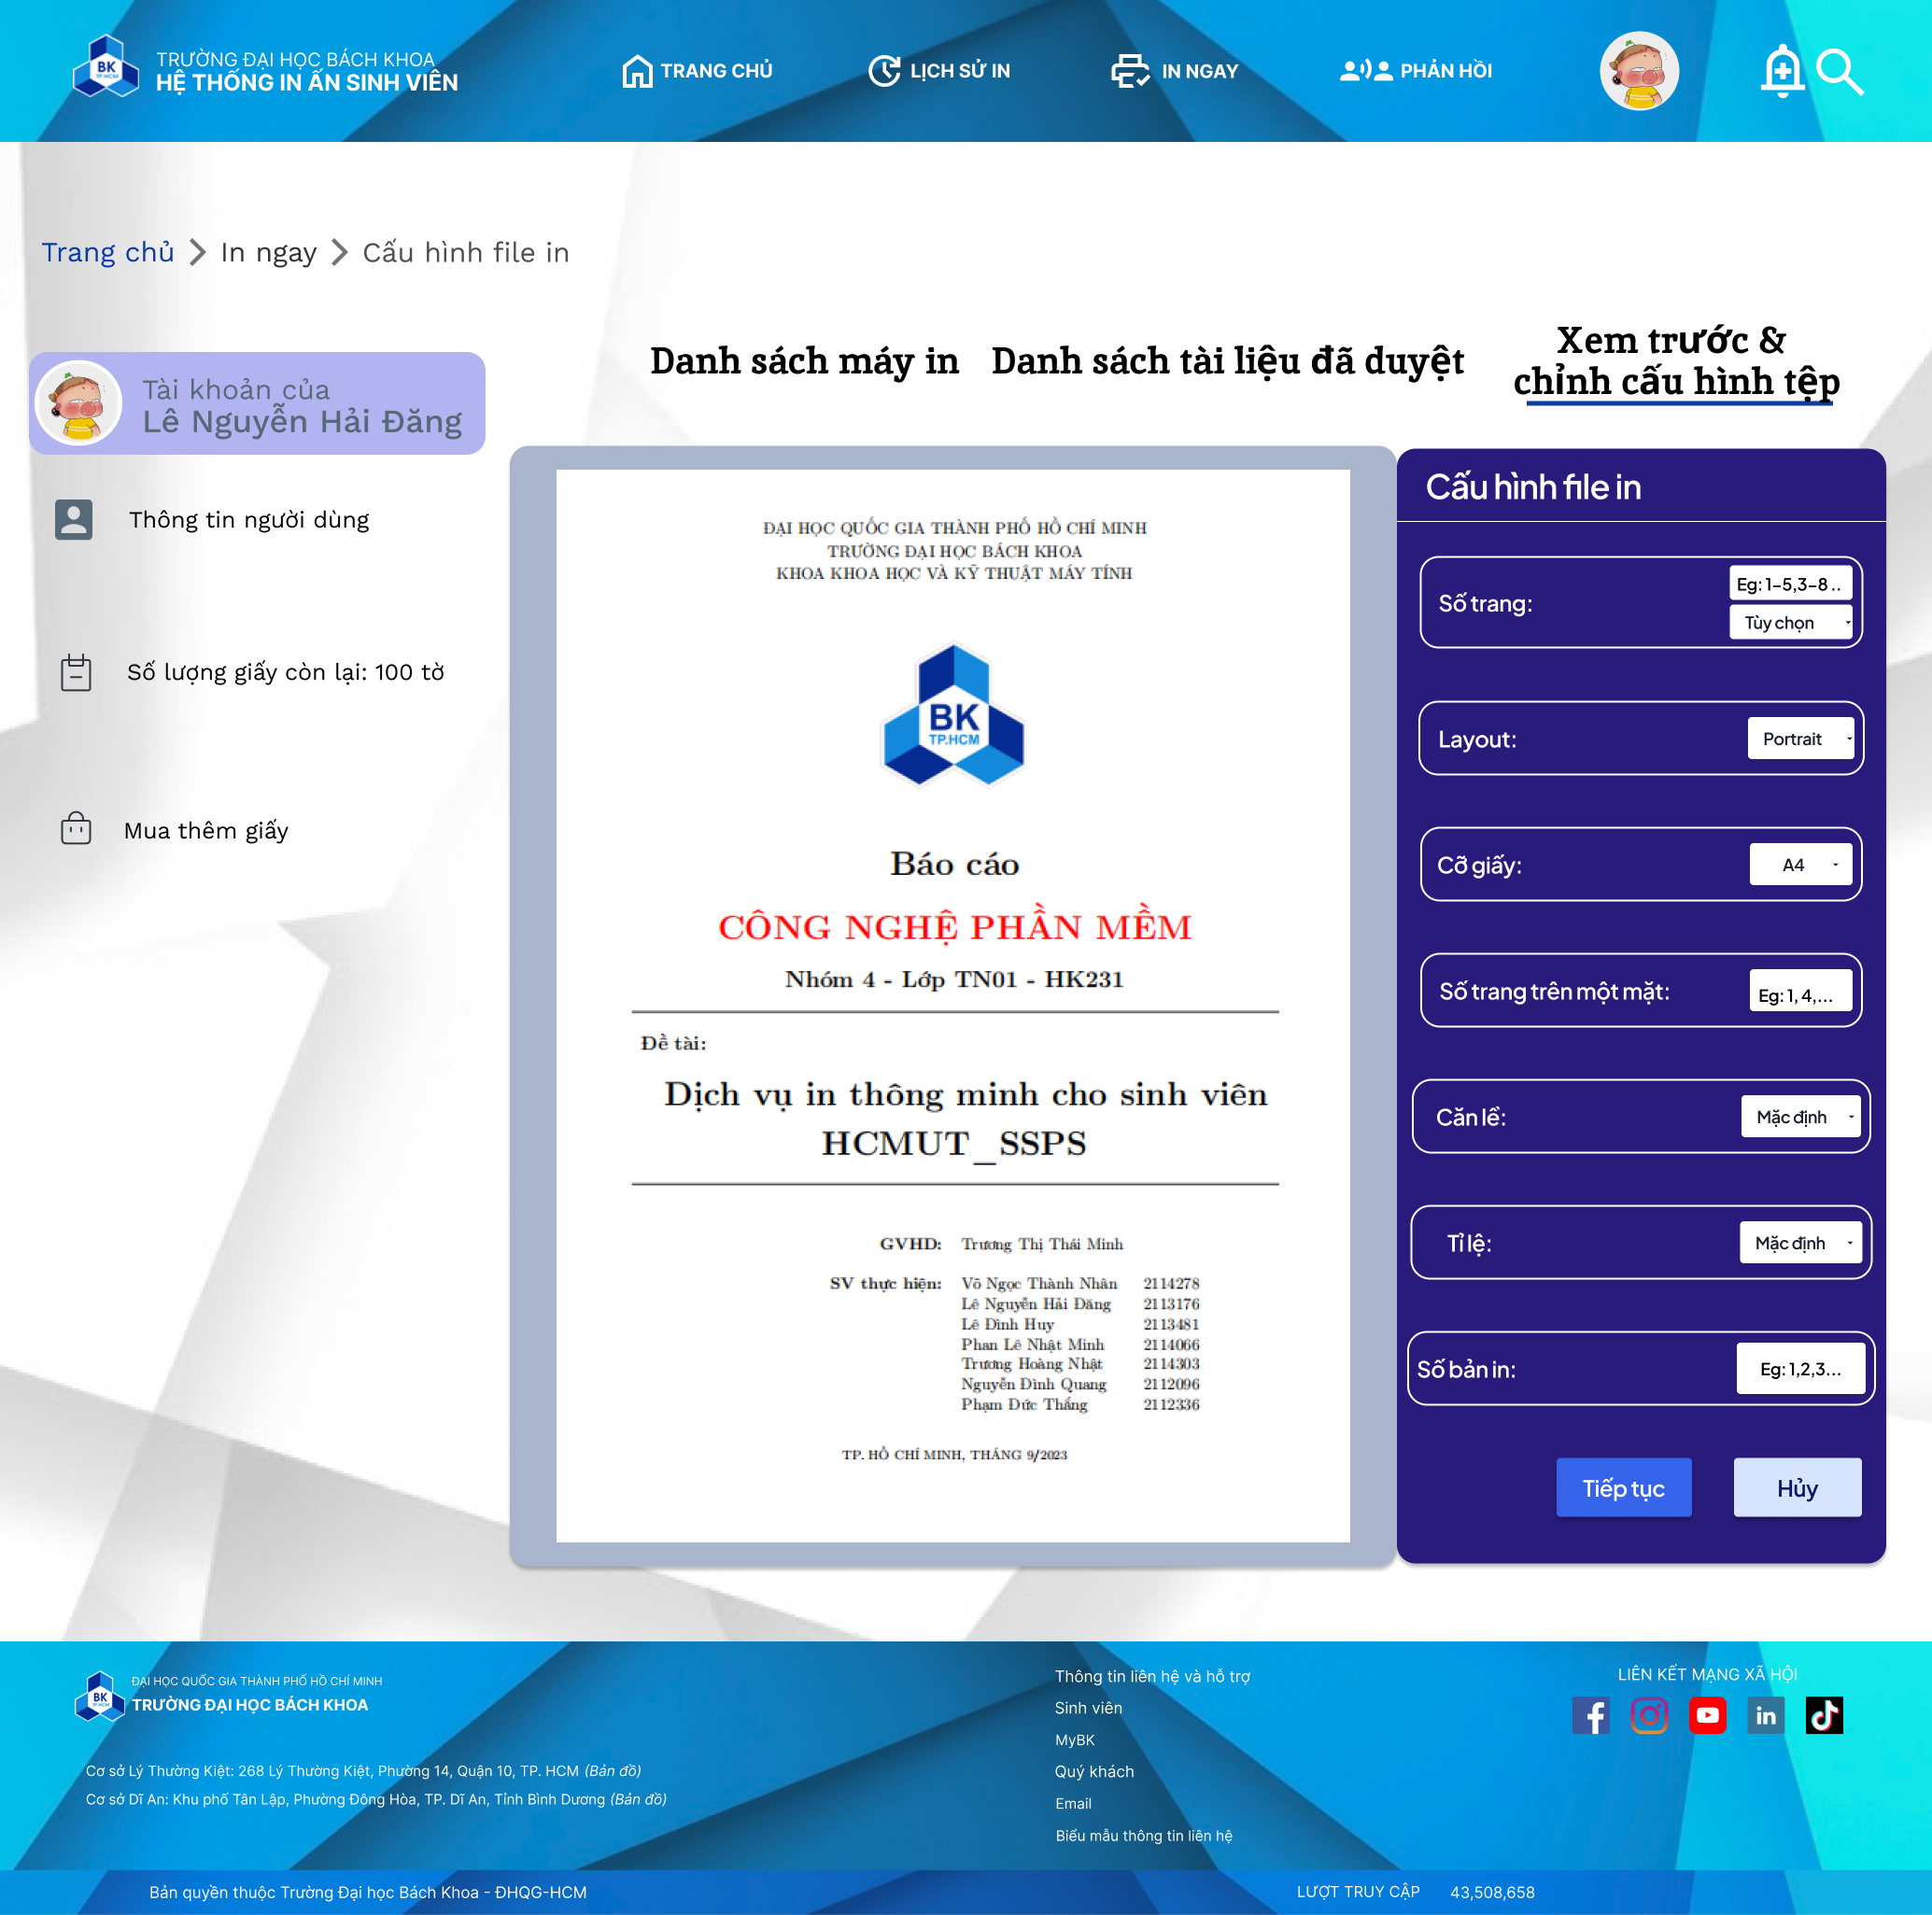
\includegraphics[width=1\textwidth]{Images/Figma/Config.png}
        \caption{Giao diện cài đặt cấu hình file in}
        \label{fig:arch}
    \end{center}
\end{figure}
$\indent$- Khi hoàn tất cấu hình, bấm tiếp tục để xem trang trước khi in.
\begin{figure}[H] 
    \begin{center}
        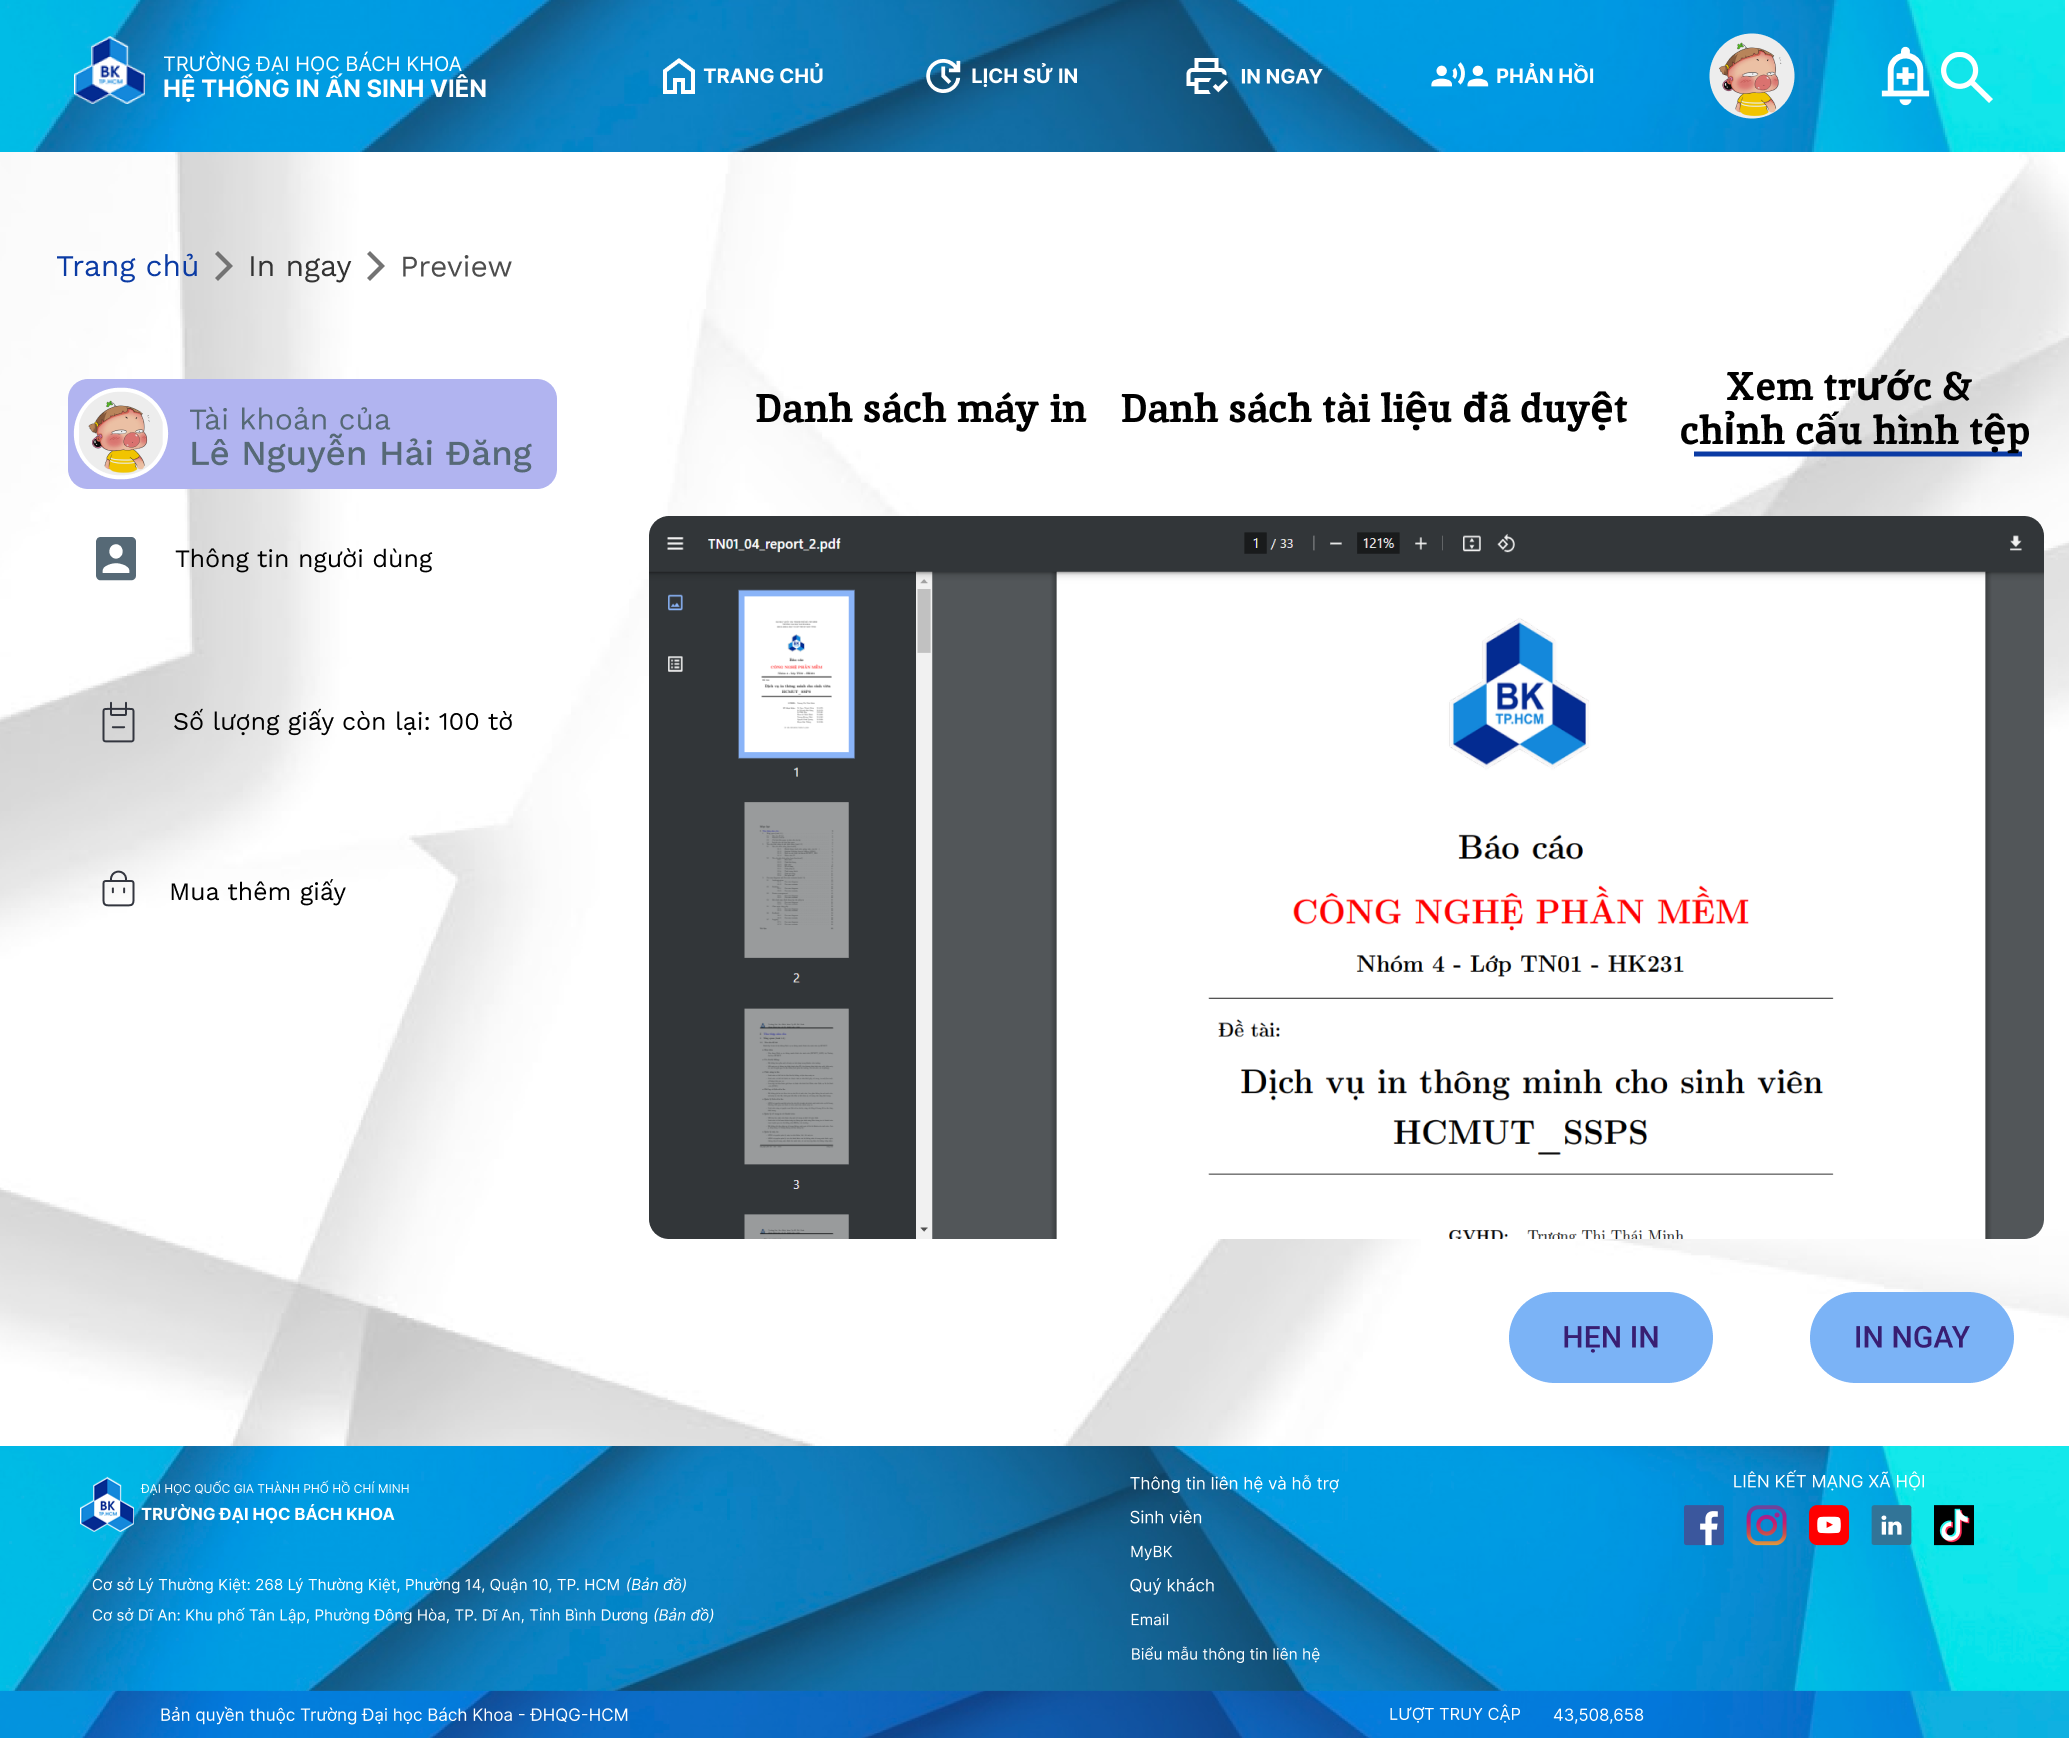
\includegraphics[width=1\textwidth]{Images/Figma/Preview.png}
        \caption{Giao diện xem trước tài liệu in của khách hàng}
        \label{fig:arch}
    \end{center}
\end{figure}

\subsubsection{Quản lý máy in}
\begin{figure}[H]
    \begin{center}
        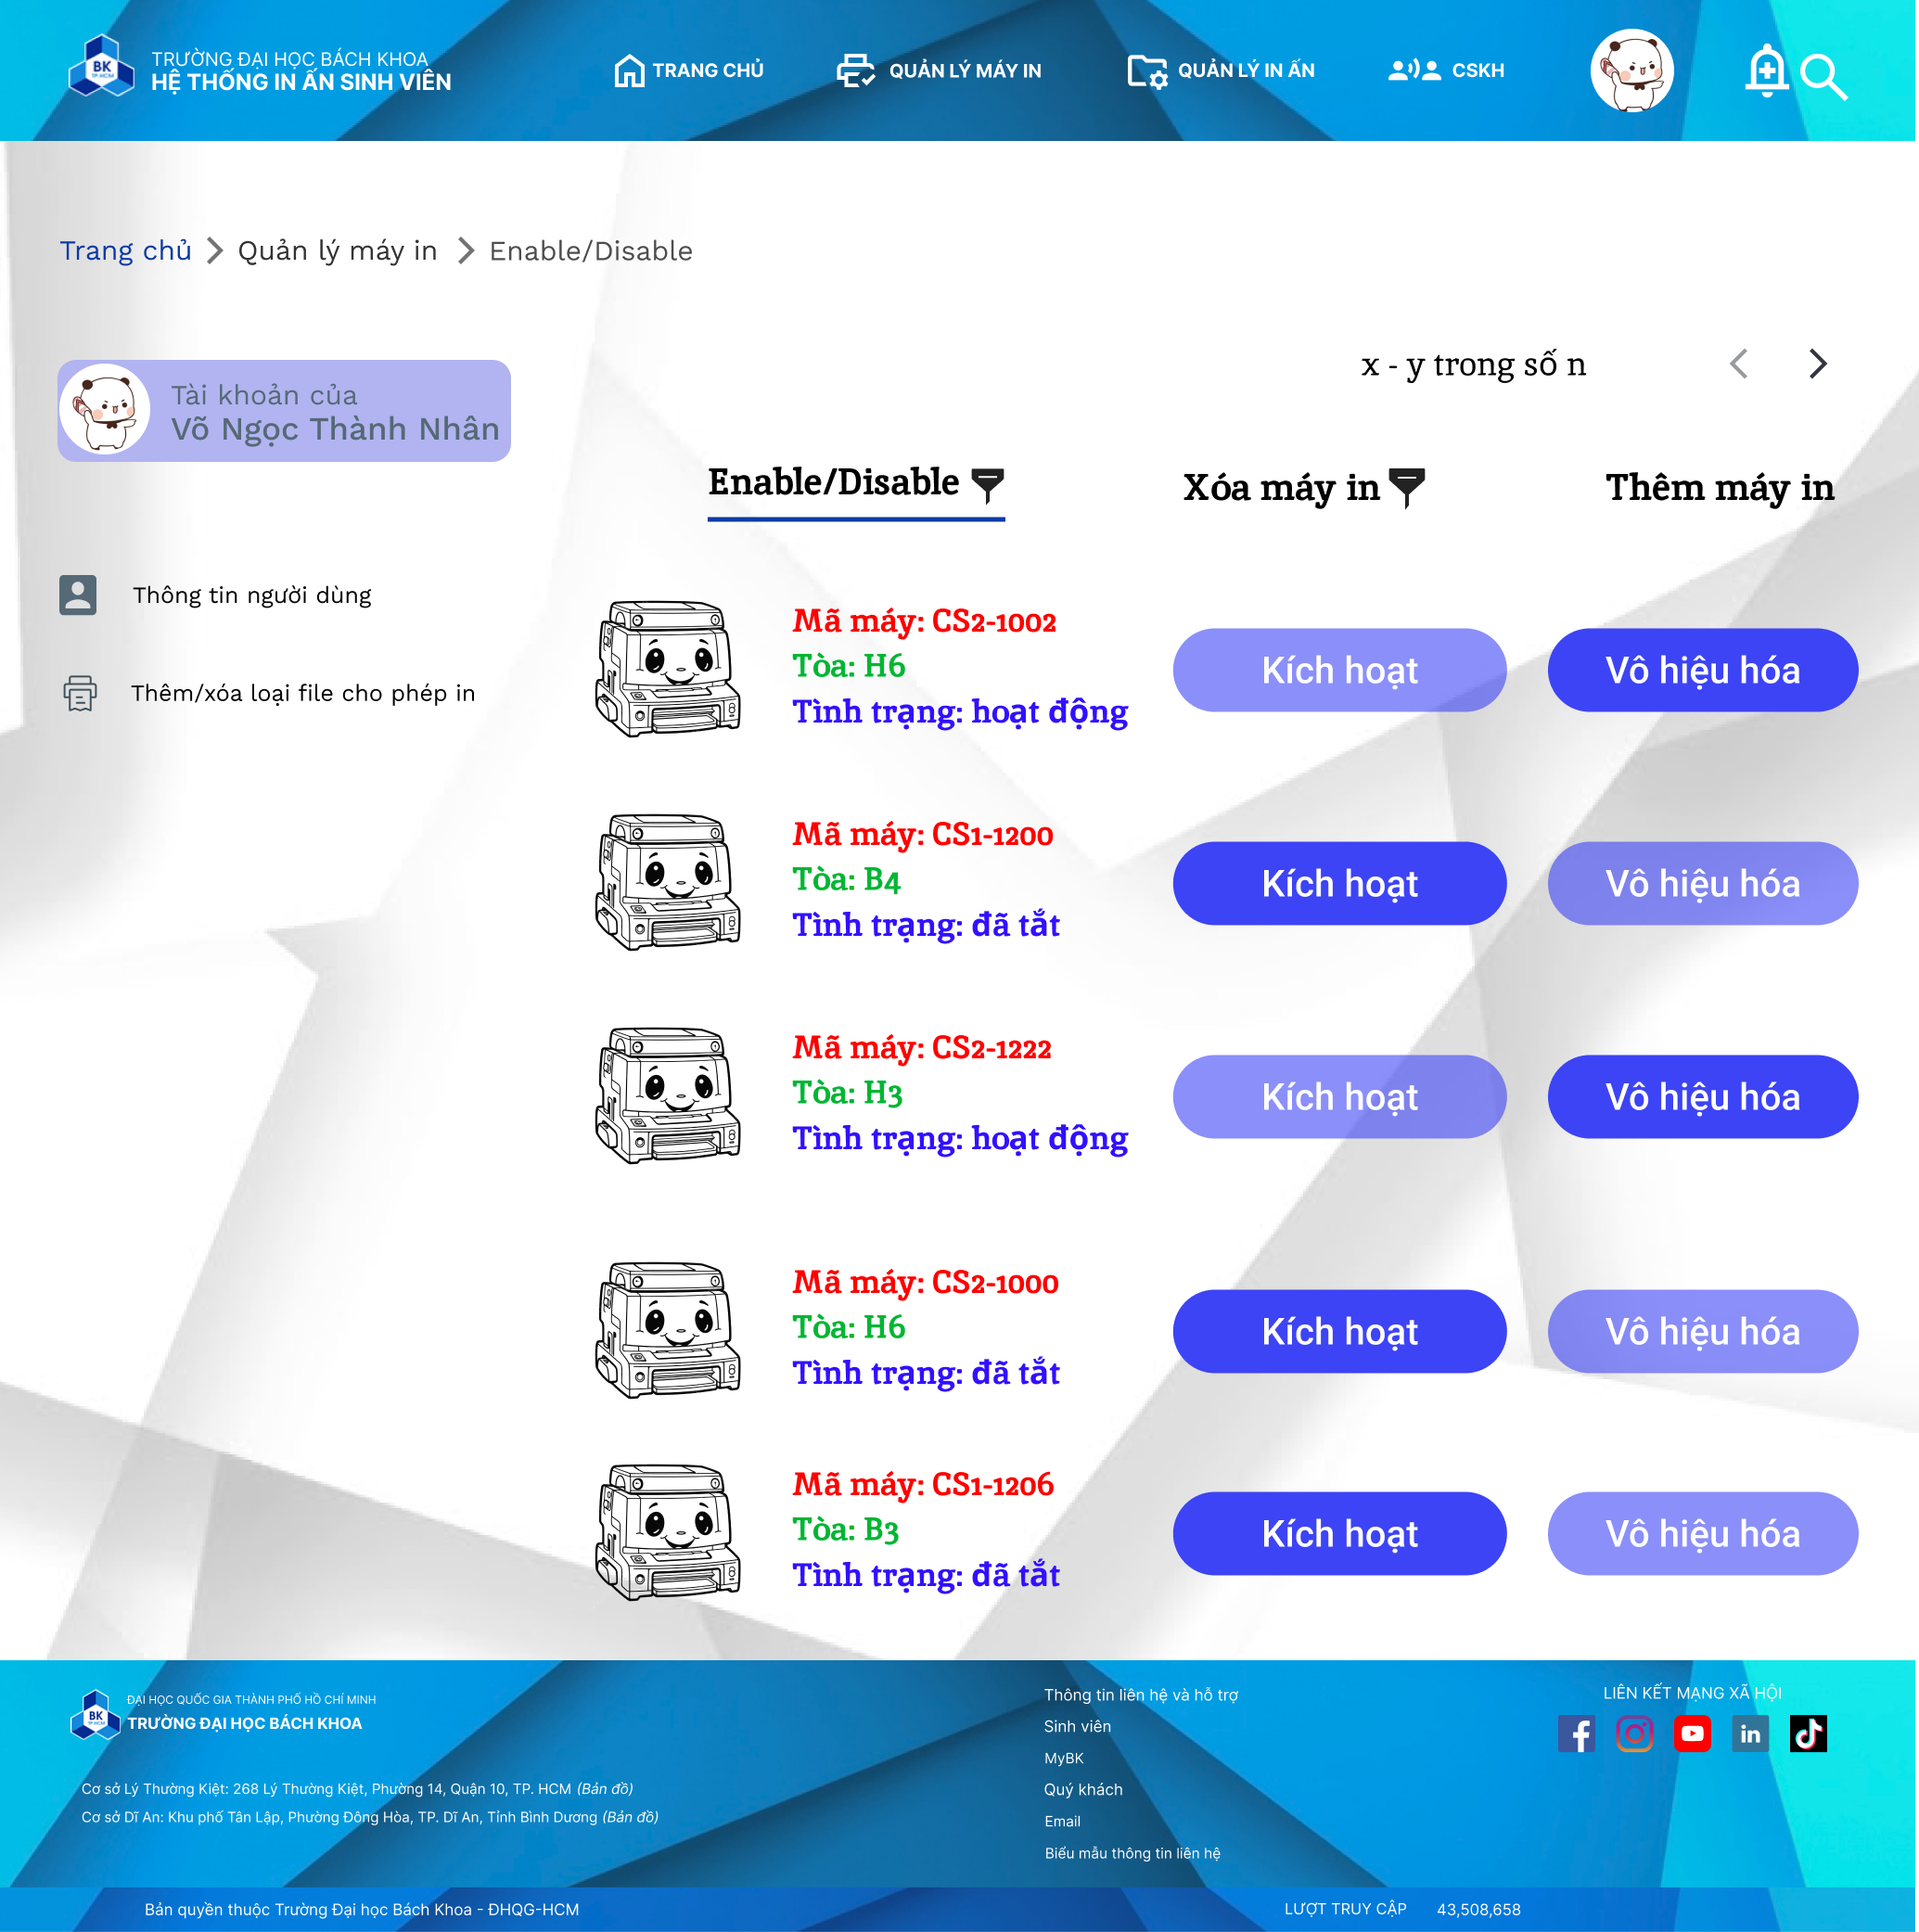
\includegraphics[width=1\textwidth]{Images/Figma/Enable-disable.png}
        \caption{Giao diện Kích hoạt-Vô hiệu hóa máy in của SPSO}
        \label{fig:arch}
    \end{center}
\end{figure}
\begin{figure}[H]
    \begin{center}
        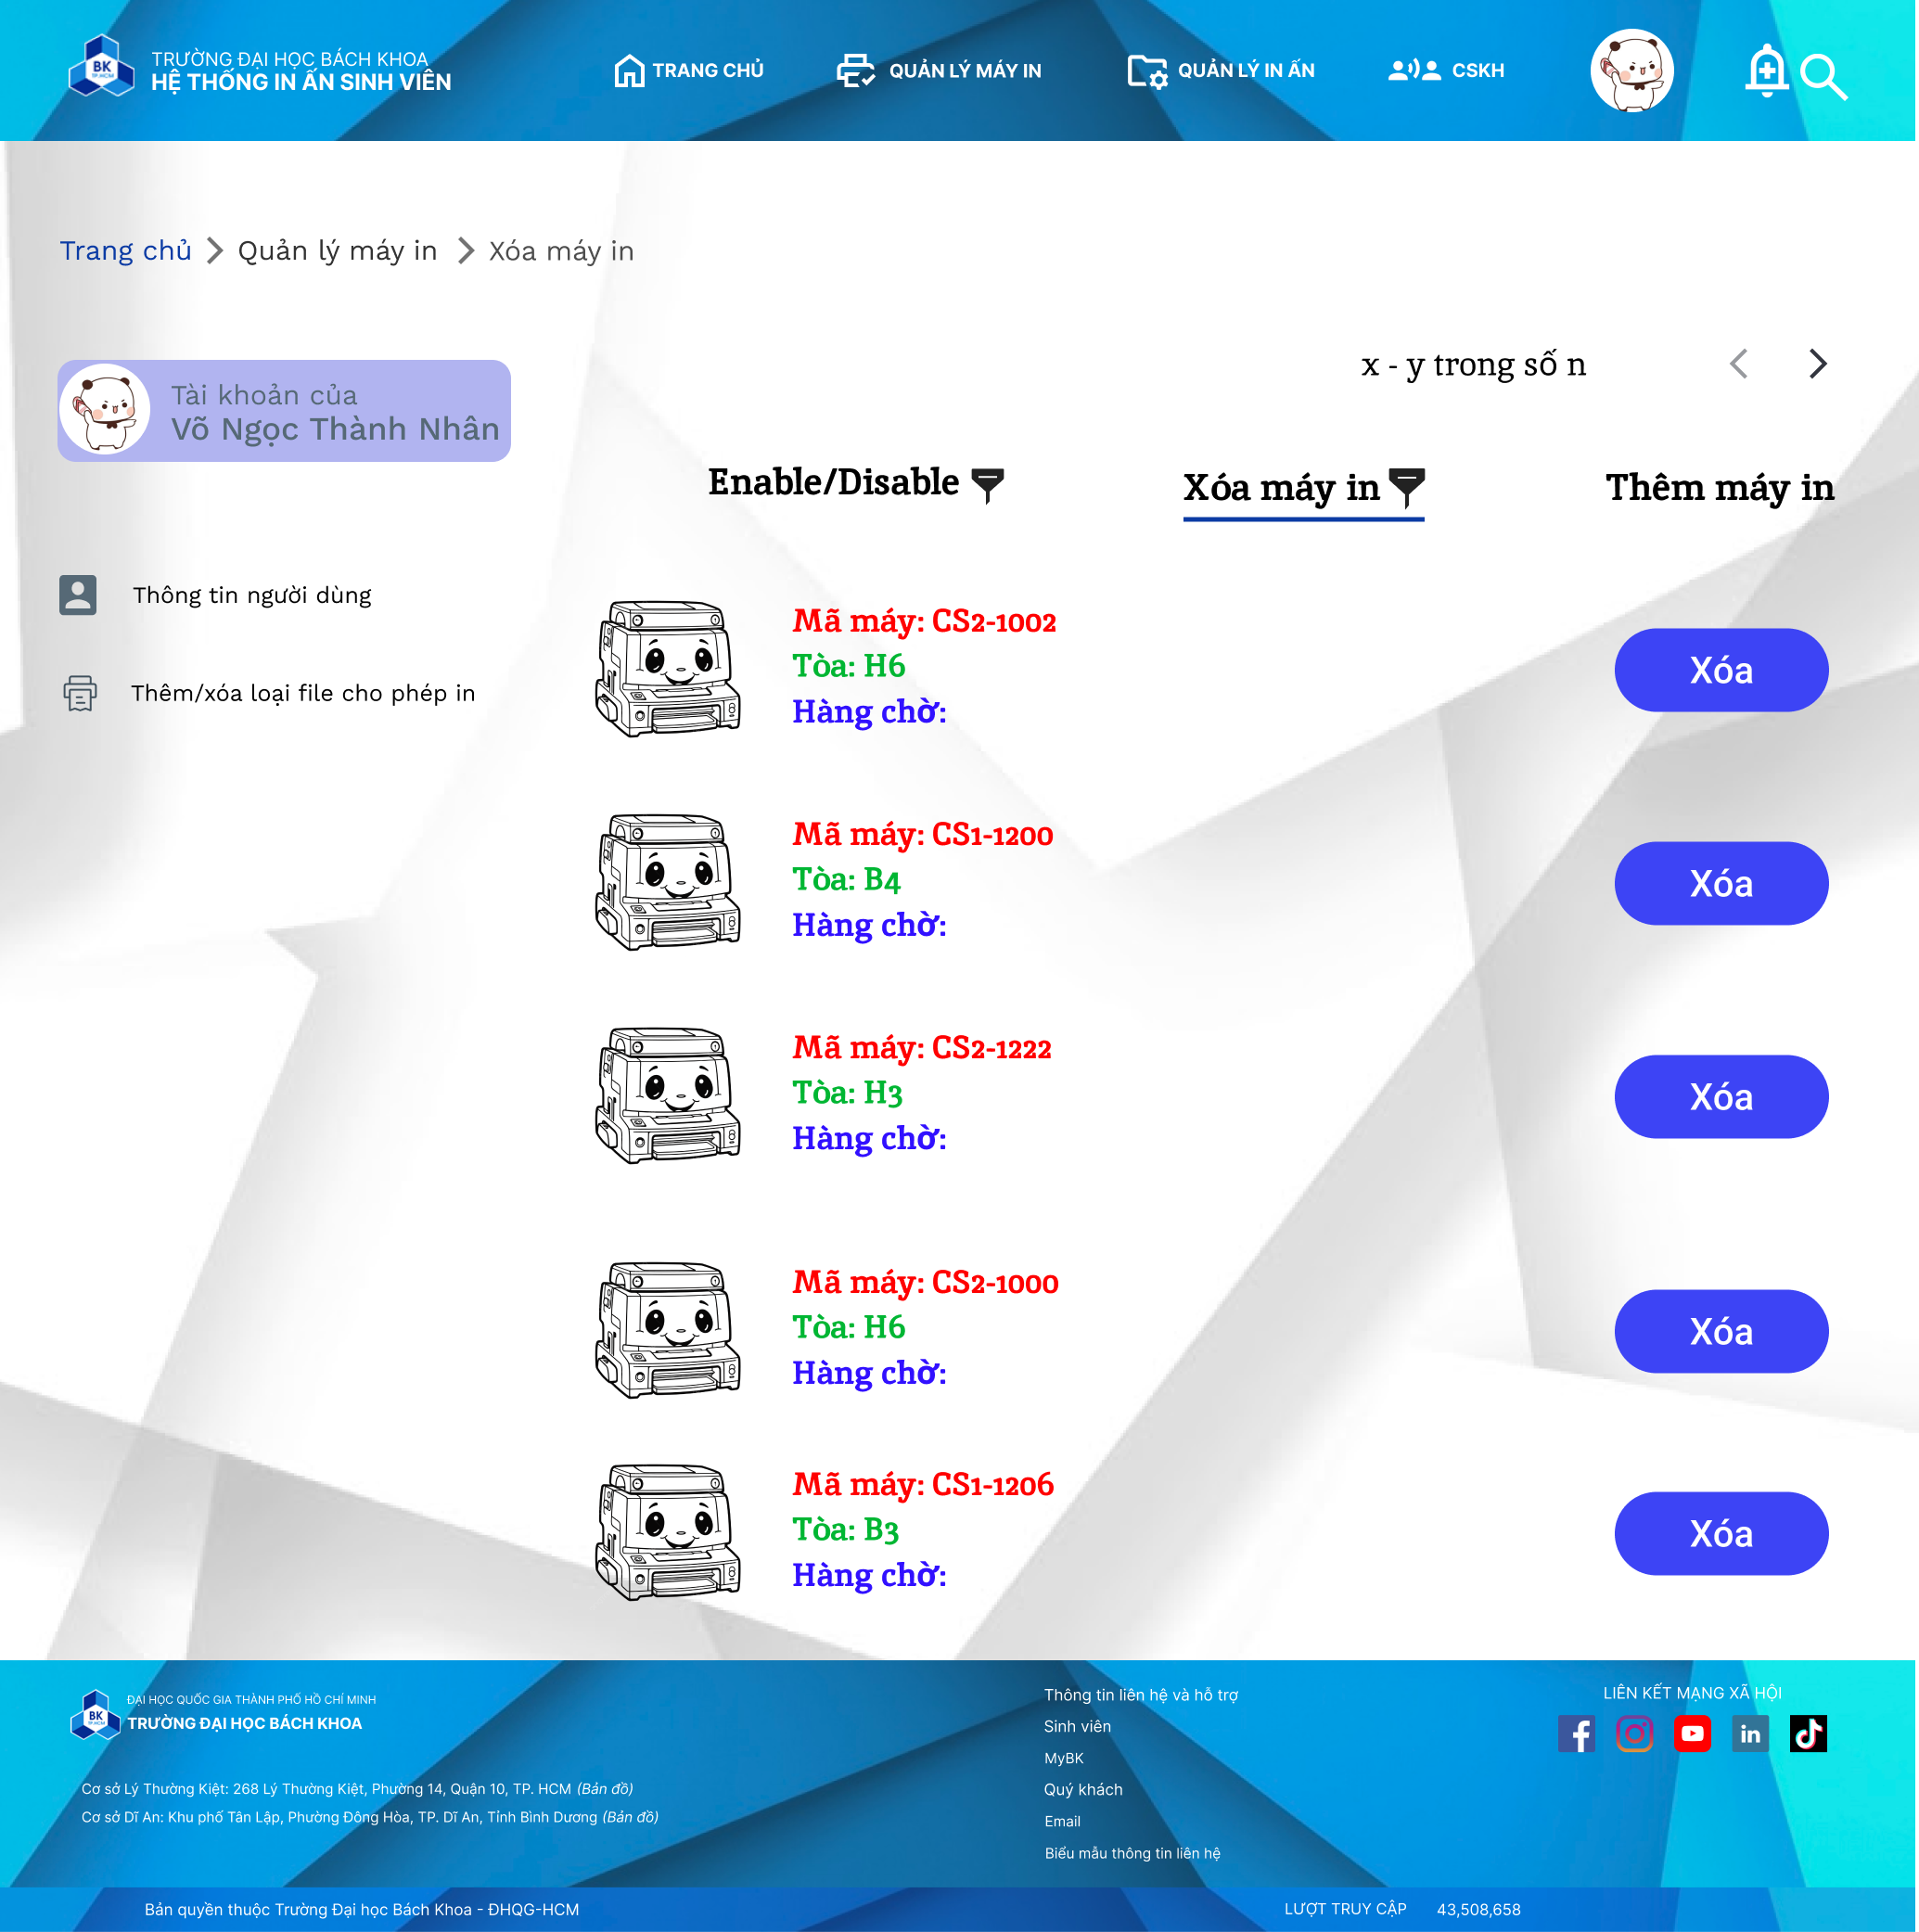
\includegraphics[width=1\textwidth]{Images/Figma/Xóa máy in.png}
        \caption{Giao diện Xóa máy in của SPSO}
        \label{fig:arch}
    \end{center}
\end{figure}
\begin{figure}[H]
    \begin{center}
        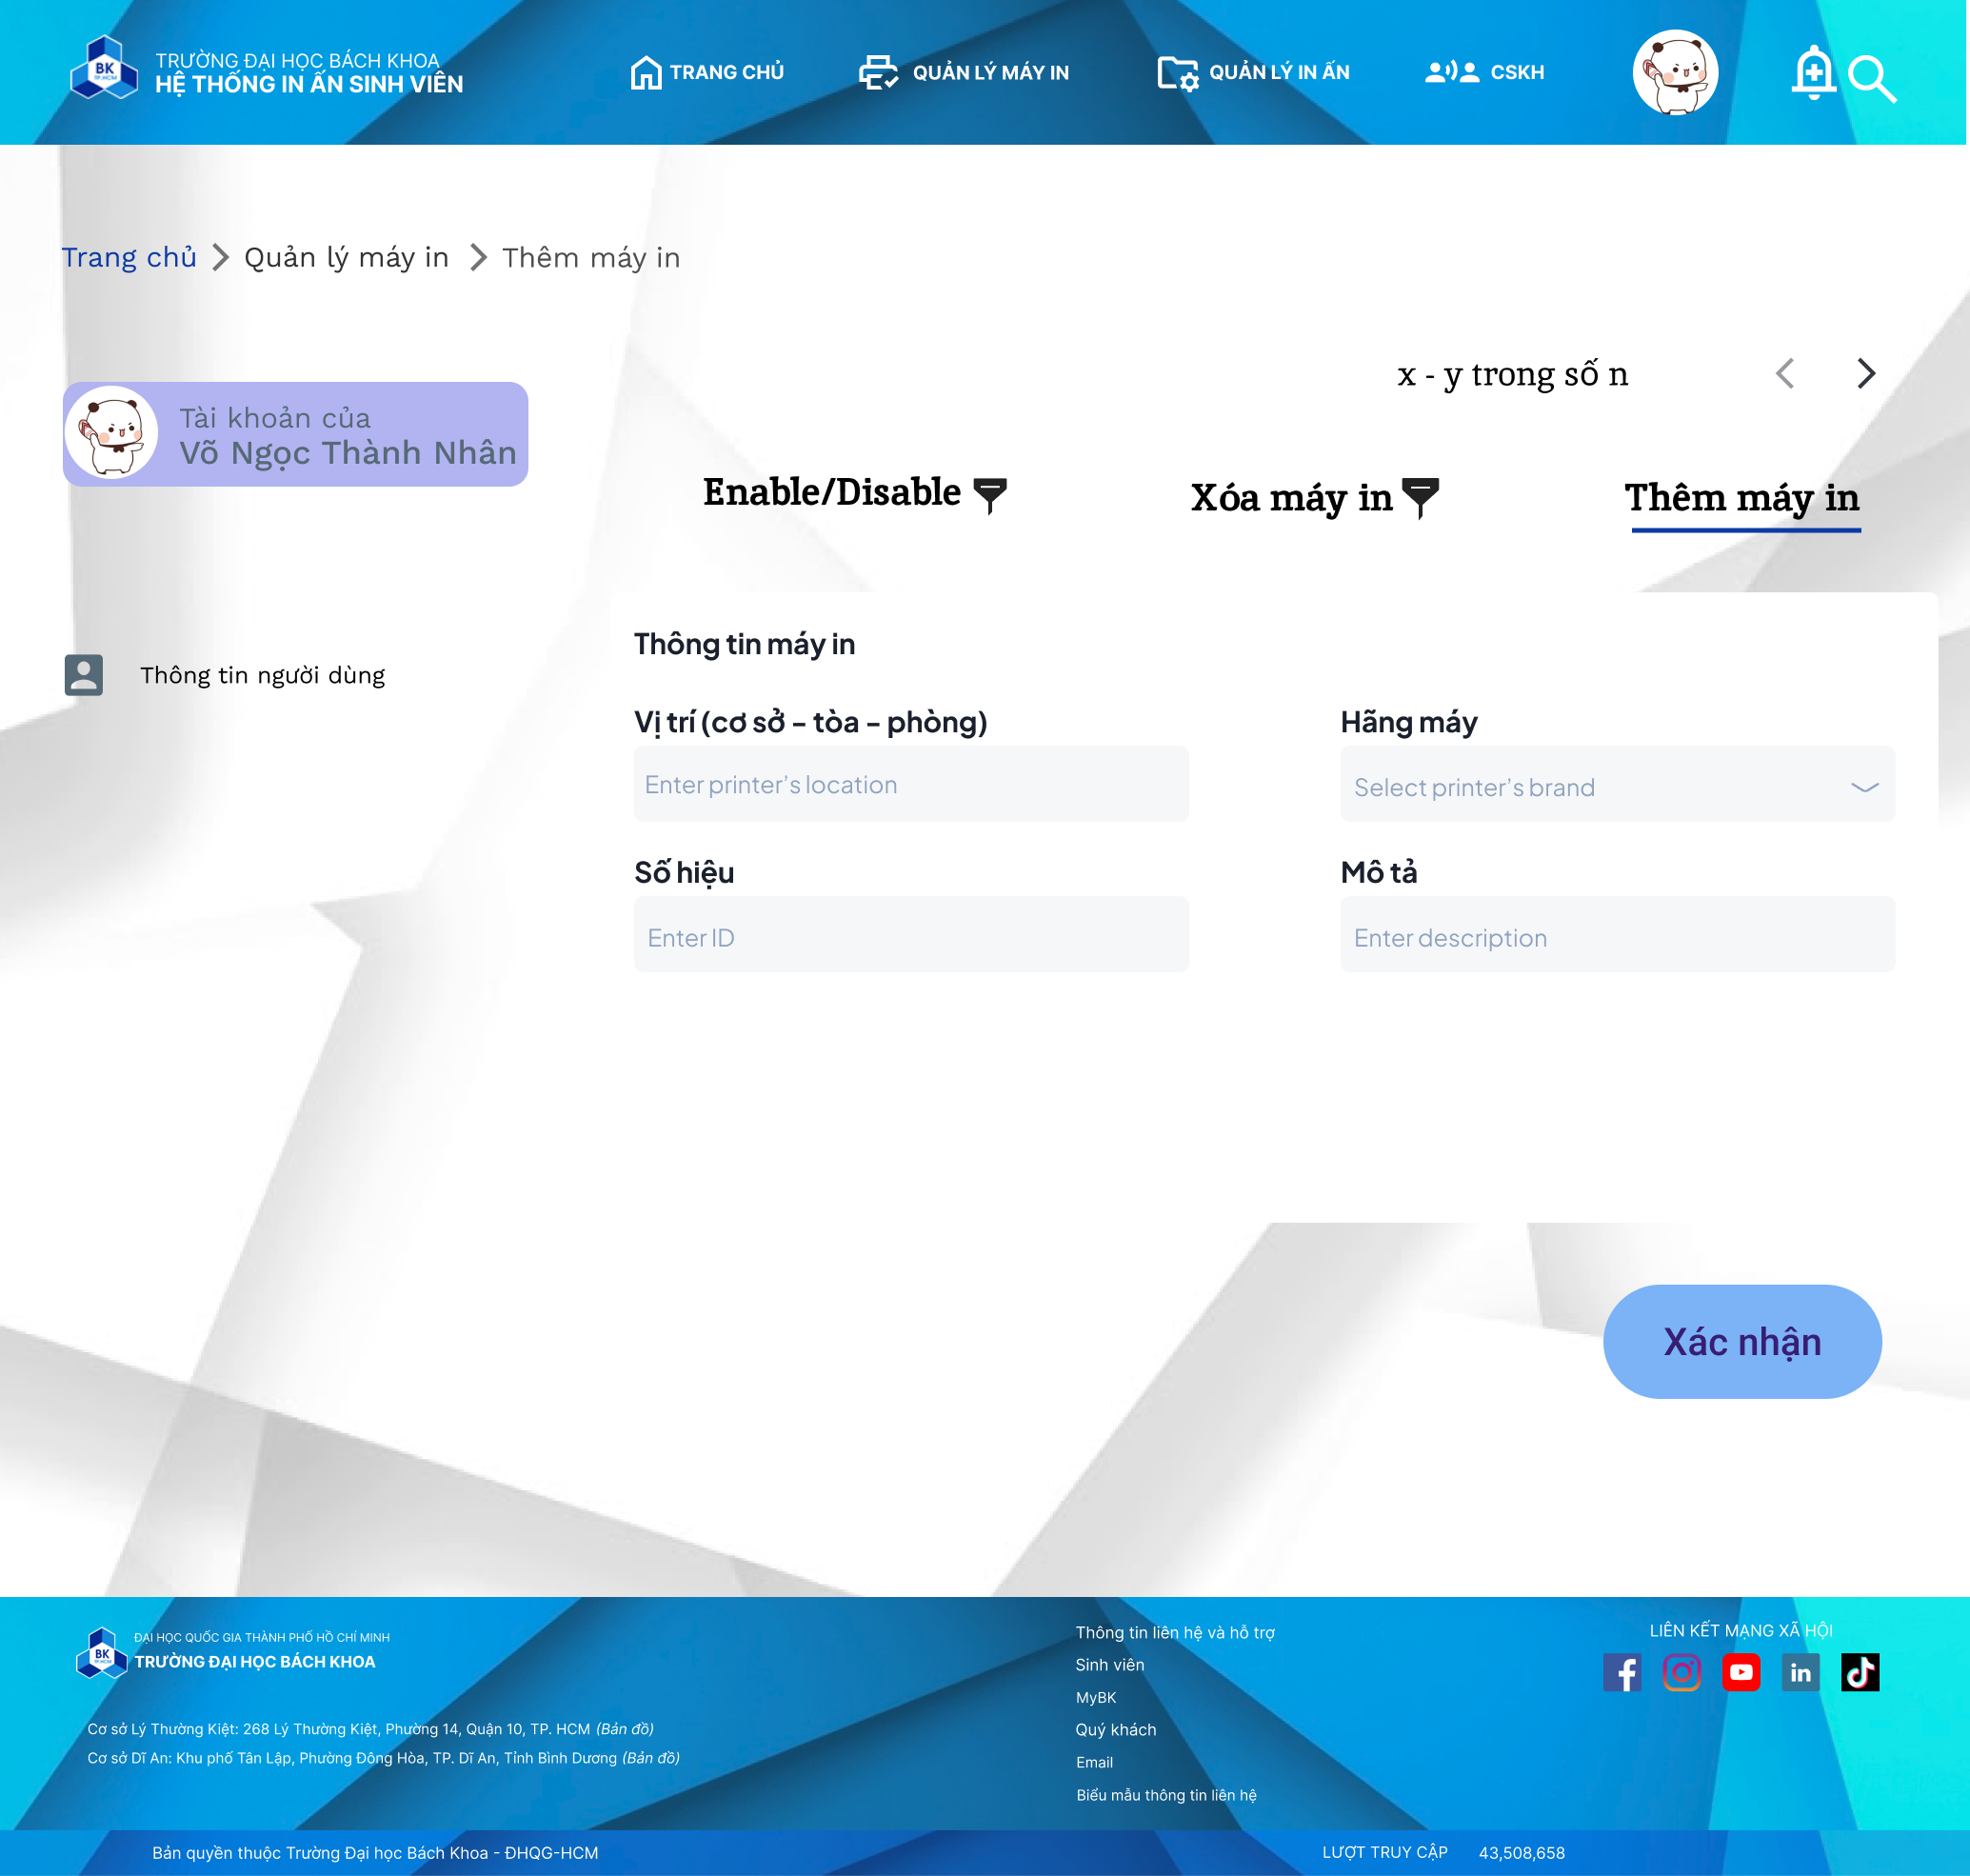
\includegraphics[width=1\textwidth]{Images/Figma/Thêm máy in.png}
        \caption{Giao diện Thêm máy in của SPSO}
        \label{fig:arch}
    \end{center}
\end{figure}
\subsubsection{Quản lý in ấn}
\begin{figure}[H]
    \begin{center}
        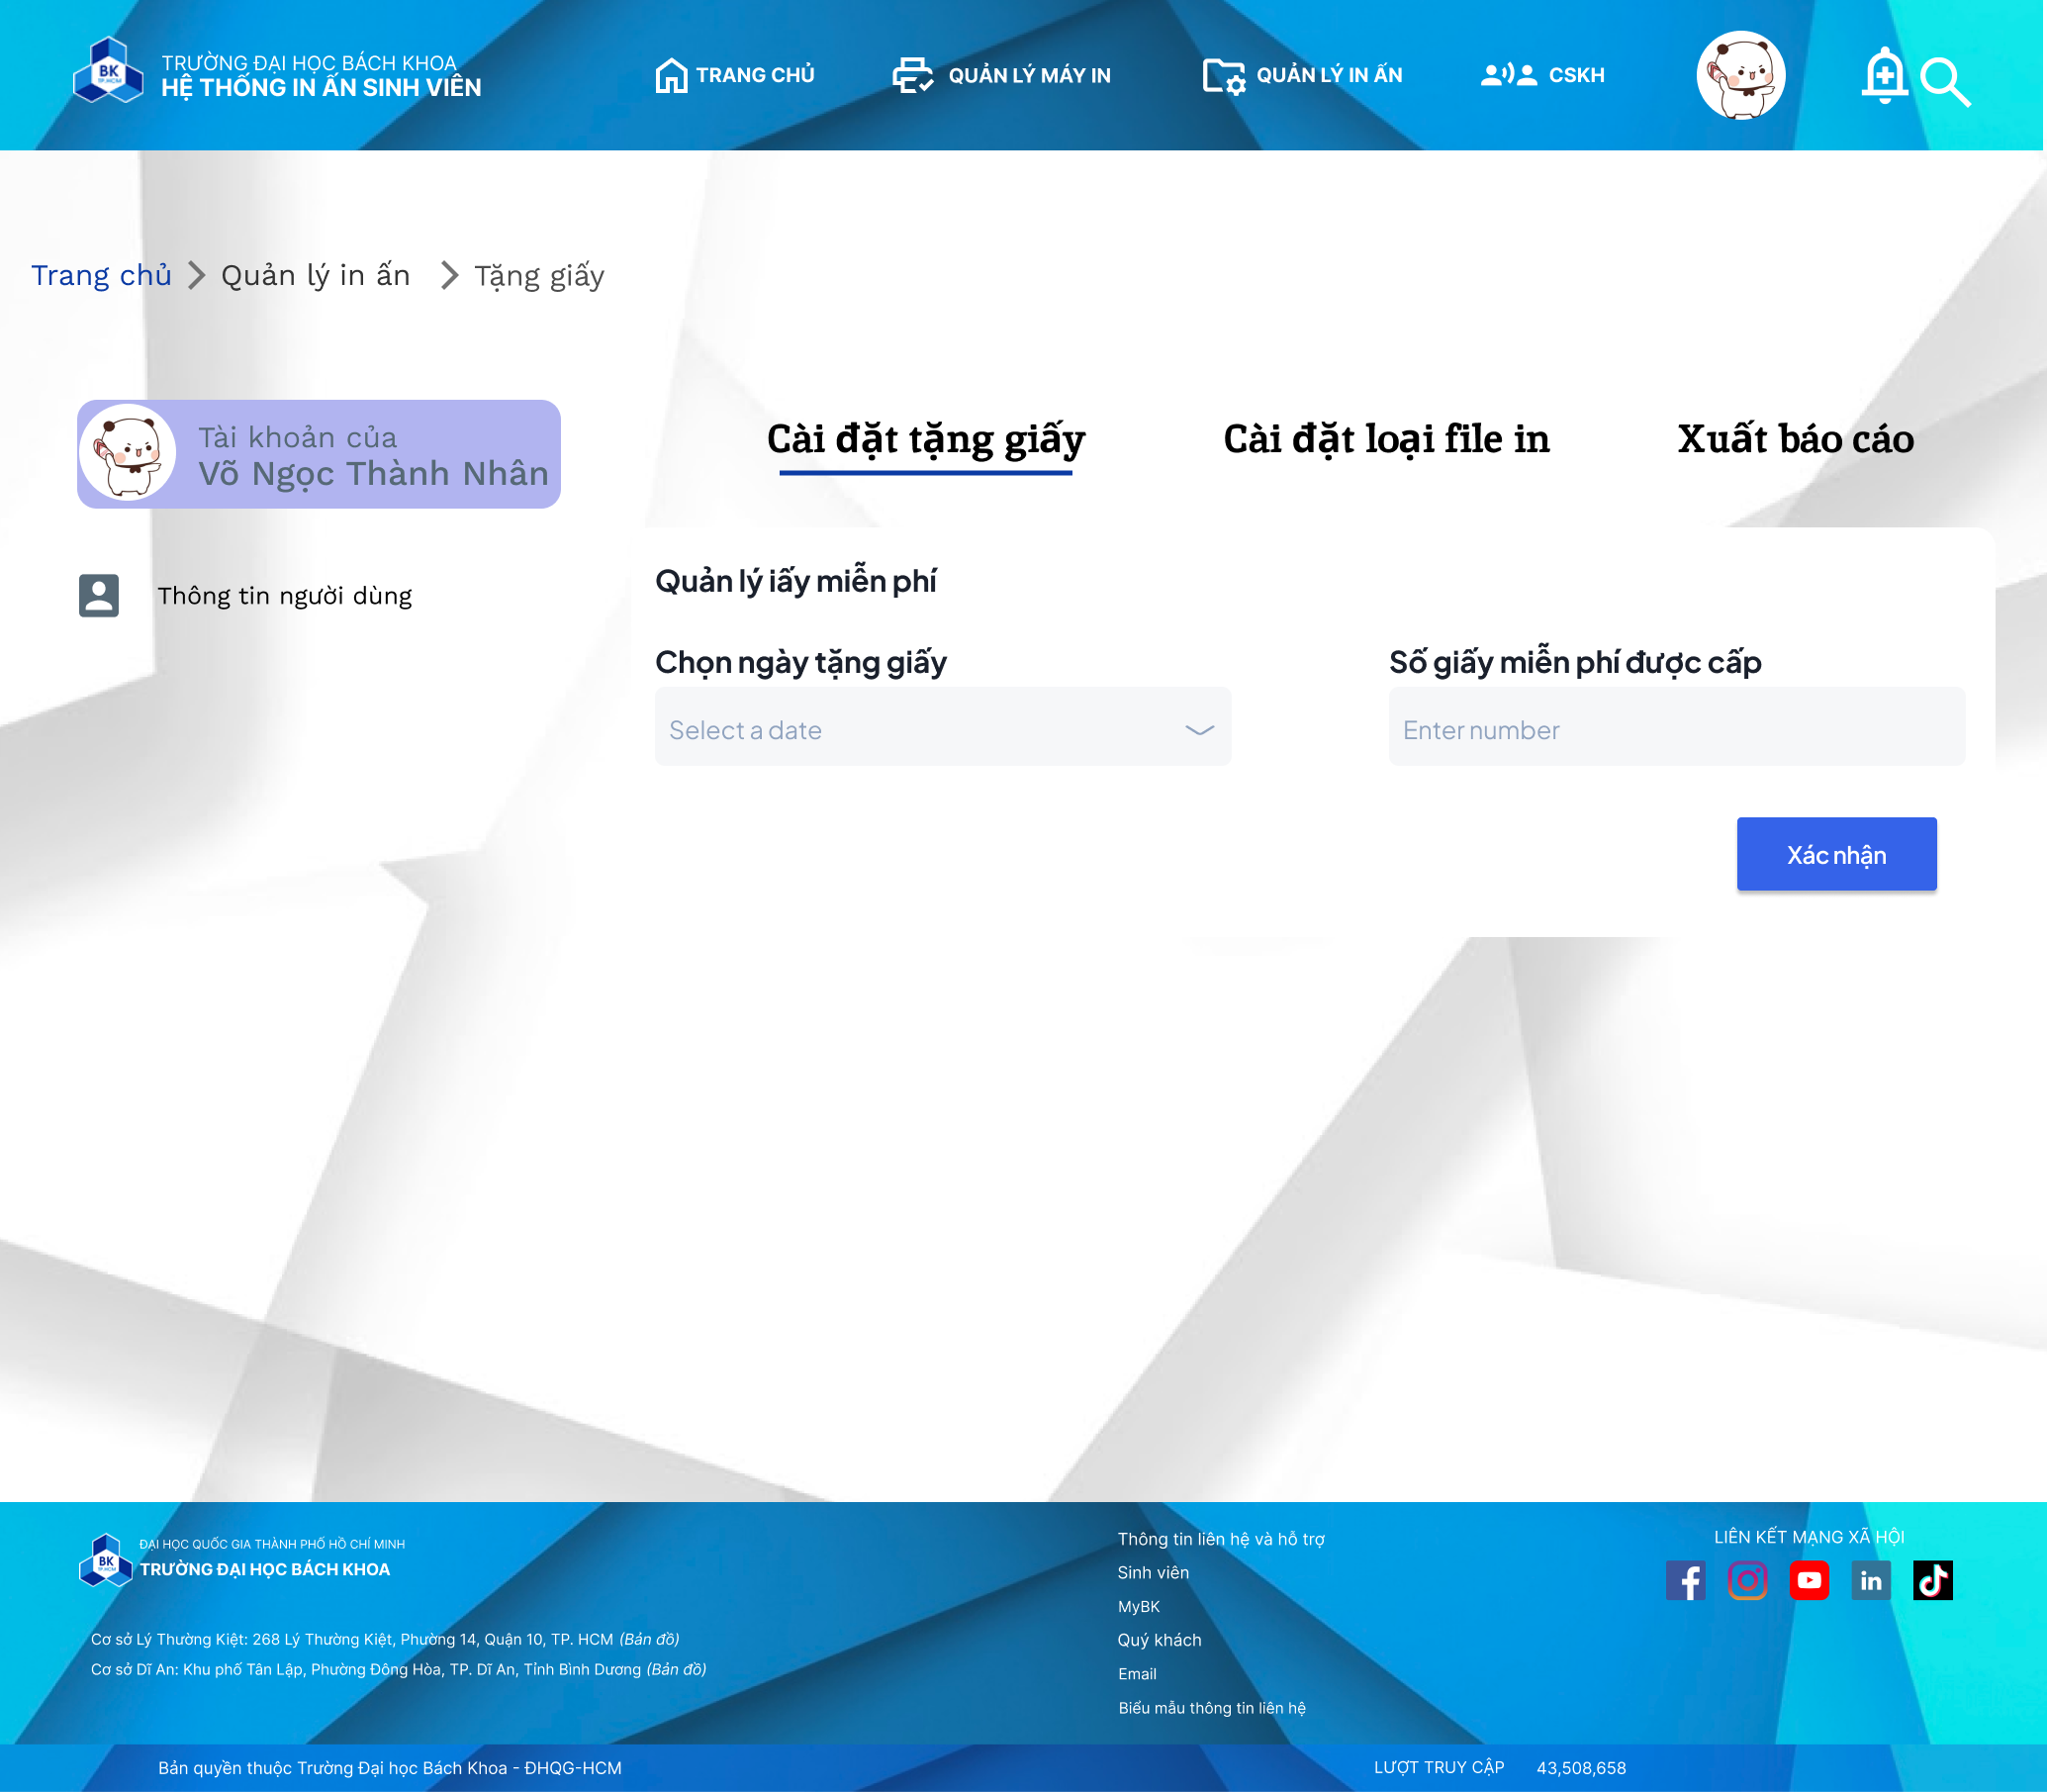
\includegraphics[width=1\textwidth]{Images/Figma/Cài đặt tặng giấy.png}
        \caption{Giao diện Thay đổi ngày nhận trang in và số lượng trang in}
        \label{fig:arch}
    \end{center}
\end{figure}
\subsubsection{Mua giấy}
\begin{figure}[H]
    \begin{center}
        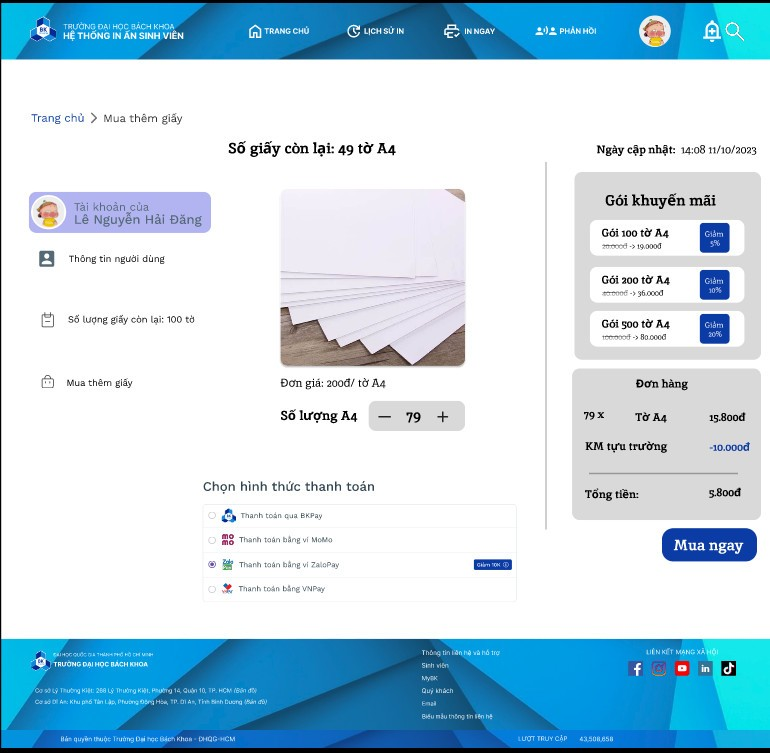
\includegraphics[width=1\textwidth]{Images/Figma/buy_main.png}
        \caption{Giao diện mua giấy của khách hàng.}
        \label{fig:arch}
    \end{center}
\end{figure}
\begin{figure}[H]
    \begin{center}
        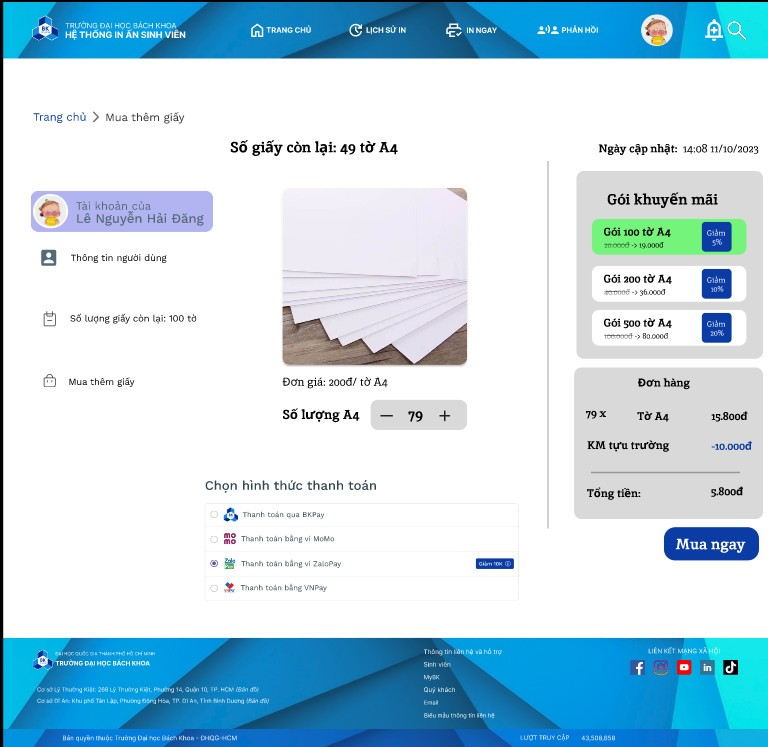
\includegraphics[width=1\textwidth]{Images/Figma/buy_package.png}
        \caption{Giao diện khi khách hàng chọn các gói khuyến mãi.}
        \label{fig:arch}
    \end{center}
\end{figure}
\begin{figure}[H]
    \begin{center}
        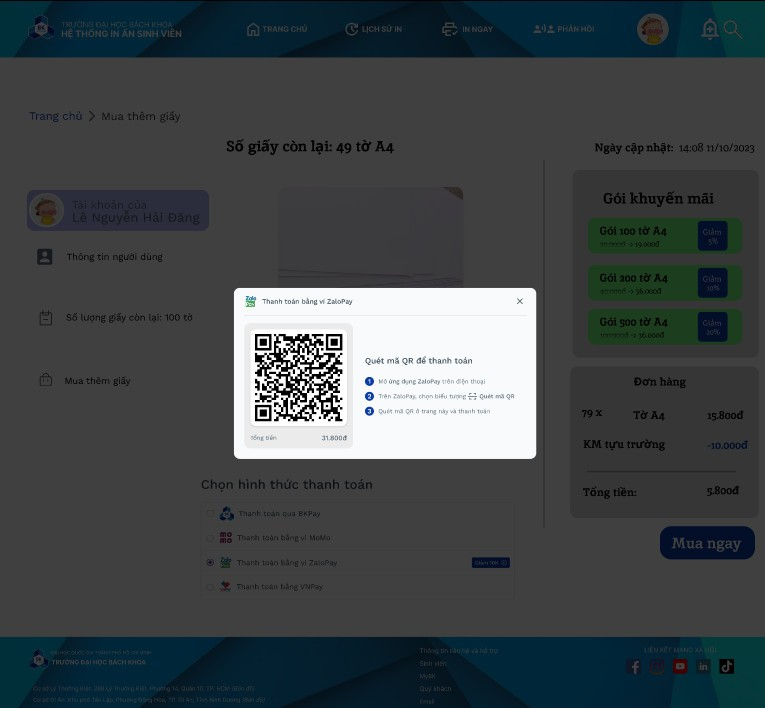
\includegraphics[width=1\textwidth]{Images/Figma/zalopay.png}
        \caption{Giao diện thanh toán bằng mã QR.}
        \label{fig:arch}
    \end{center}
\end{figure}
\subsubsection{Lịch sử in}
\begin{figure}[H]
    \begin{center}
        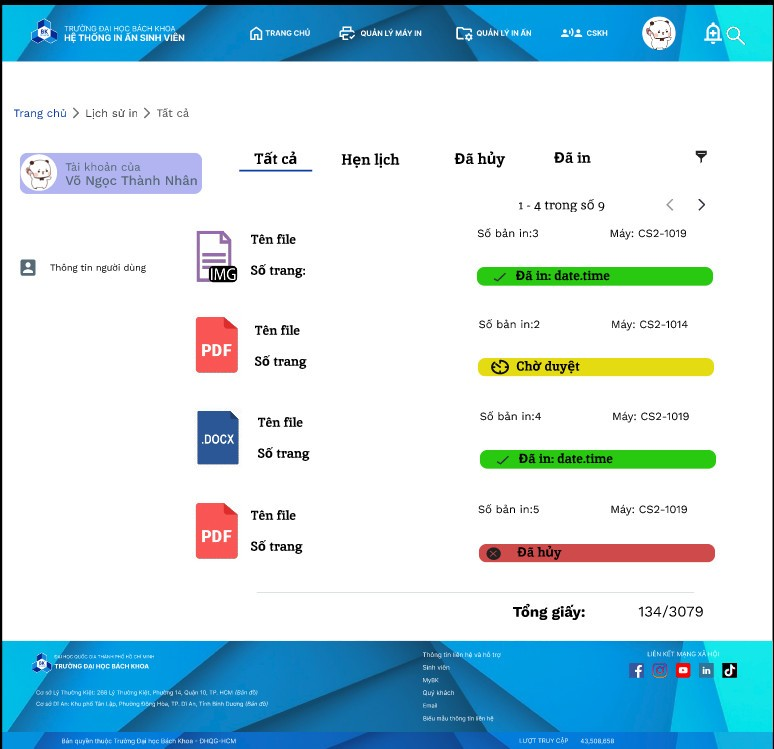
\includegraphics[width=1\textwidth]{Images/Figma/history_main.png}
        \caption{Giao diện xem lịch sử in của SPSO}
        \label{fig:arch}
    \end{center}
\end{figure}
\begin{figure}[H]
    \begin{center}
        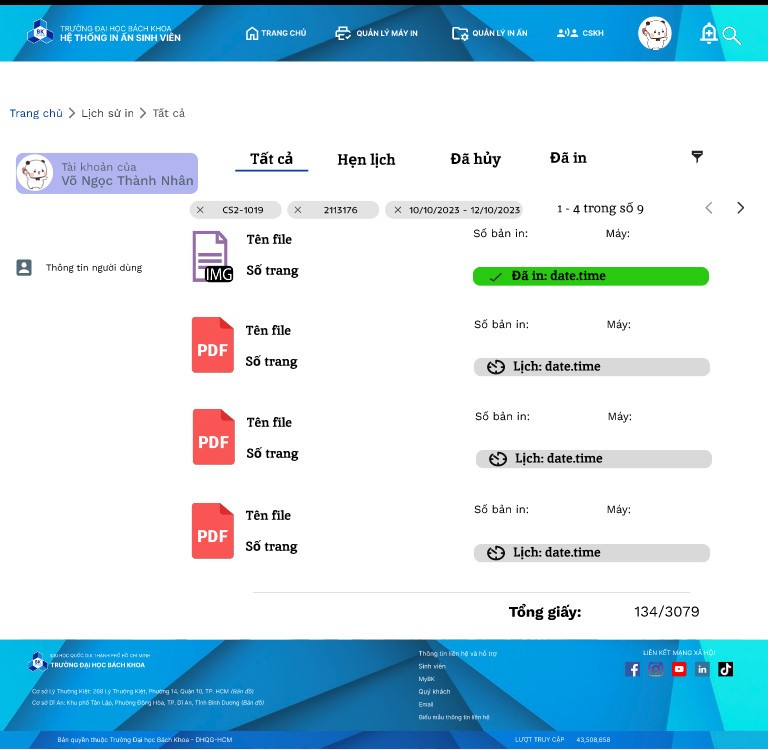
\includegraphics[width=1\textwidth]{Images/Figma/history_filter.png}
        \caption{Giao diện xem lịch sử in của SPSO khi chọn ngày, mã máy in, mã số sinh viên}
        \label{fig:arch}
    \end{center}
\end{figure}
\subsubsection{Phản hồi - CSKH}
\begin{figure}[H]
    \begin{center}
        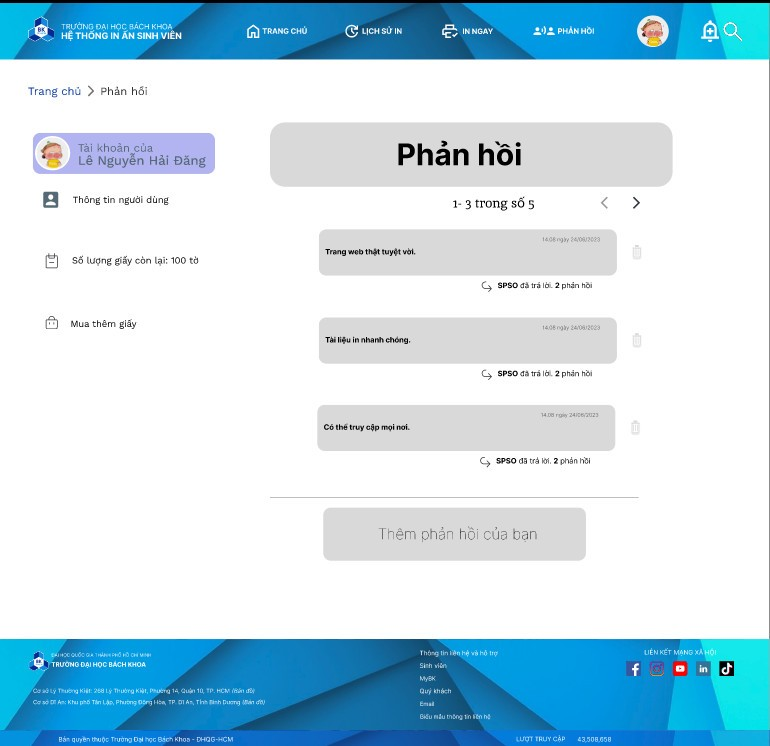
\includegraphics[width=1\textwidth]{Images/Figma/comment.png}
        \caption{Giao diện phản hồi cuả khách hàng.}
        \label{fig:arch}
    \end{center}
\end{figure}
\begin{figure}[H]
    \begin{center}
        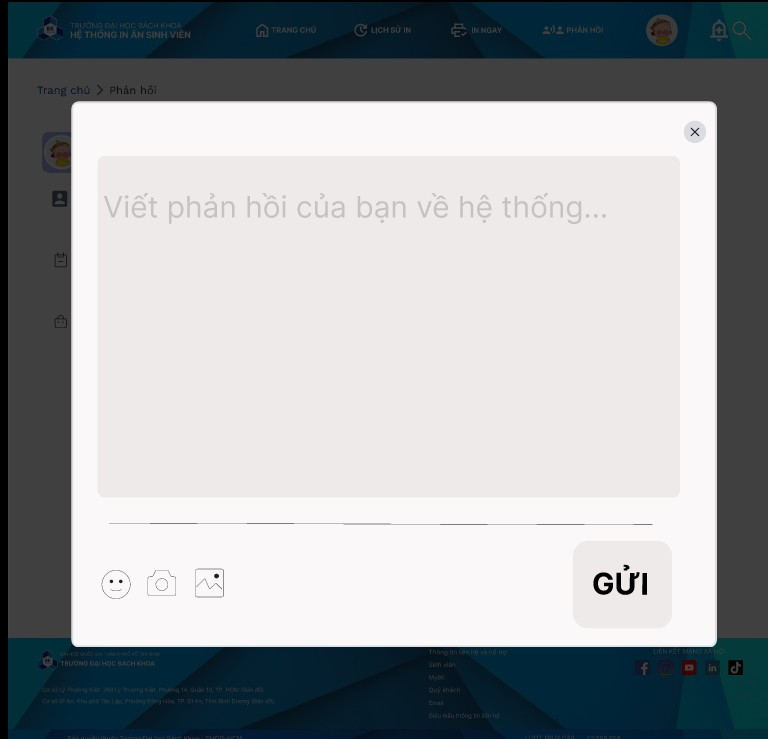
\includegraphics[width=1\textwidth]{Images/Figma/add_cmt.png}
        \caption{Giao diện khi muốn thêm phản hồi.}
        \label{fig:arch}
    \end{center}
\end{figure}
\begin{figure}[H]
    \begin{center}
        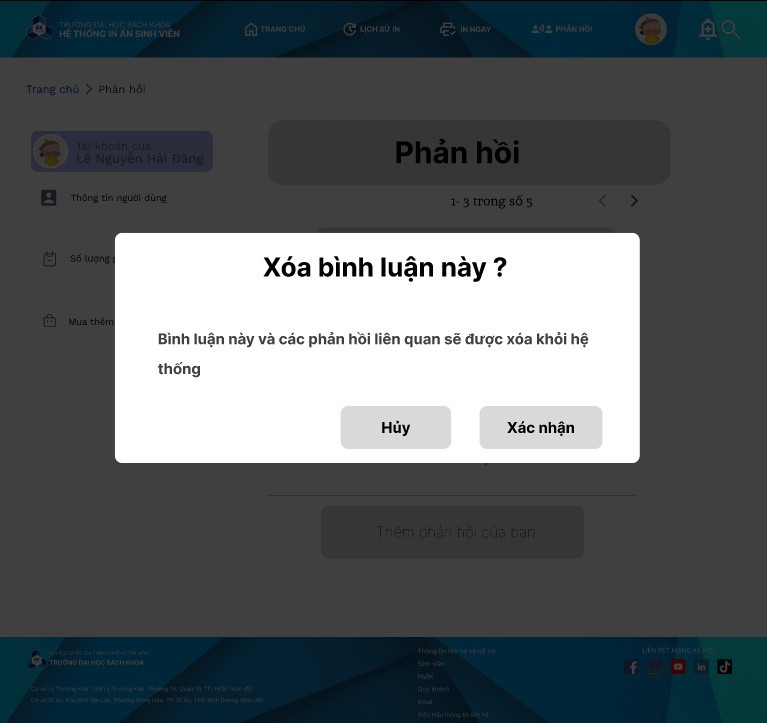
\includegraphics[width=1\textwidth]{Images/Figma/deletecmt.png}
        \caption{Giao diện khi xóa phản hồi.}
        \label{fig:arch}
    \end{center}
\end{figure}